% !TEX root =  main.tex
\chapter{Results and Discussion}
\label{chap:4}
This chapter presents the mean first-passage detection time, its variance, the ergodic product, and the detection-time distribution obtained from the Brownian dynamics simulations described in Chapter~\ref{chap:3}, across six system sizes ($N_\text{total} = 10, 30, 50, 70, 100$, and 200). Sections \ref{sec:4.1}--\ref{sec:4.5} present these results figure by figure, without interpretation. Sections \ref{sec:4.6}--\ref{sec:4.11} then interpret what the results mean for the questions posed in Section~1.3, before Section~\ref{sec:4.12} closes the chapter with a stand-alone summary. 

\section{Mean Detection Time versus Probe Number: The Caldera Shape}
\label{sec:4.1}
Across all six system sizes, $\langle T \rangle$ traces the same qualitative shape when plotted against $N_p$ which is a steep initial decline from the single-probe condition, a broad region where $\langle T \rangle$ is comparatively flat and near its minimum, and a subsequent rise as $N_p$ approaches the upper end of the sweep (Figures 4.1--4.6). This pattern holds despite $N_\text{total}$ spanning a twenty-fold range (10 to 200) and despite the absolute floor value of $\langle T \rangle$ varying considerably across systems --- from roughly 1.0\,s $N_\text{total} = 10$ down to roughly 0.3\,s at $N_\text{total} = 100$, before rising again to roughly 0.5\,s at $N_\text{total} = 200$ (a detail returned to in Section~\ref{sec:4.10}). In every system, the standard deviation (bottom panels of Figures 4.1--4.6) tracks the same qualitative shape as $\langle T \rangle$ itself: lowest near the same $N_p$ range where $\langle T \rangle$ is lowest, and widening on both flanks. None of the six systems shows a monotonically decreasing $\langle T \rangle$ over the full sample range of $N_p$, as we will see in the figures, every system eventually turns upwards before $N_p$ reaches its ceiling near $0.99 \times N_\text{total}$, confirming that the basin shape motivating the ``caldera'' name is not confined to a single system size or a narrow slice of the sweep. The six individual plots are described in turn below; their fitted optima are tabulated and discussed together in Section~\ref{sec:4.2}

\begin{figure}[htbp]
    \centering
    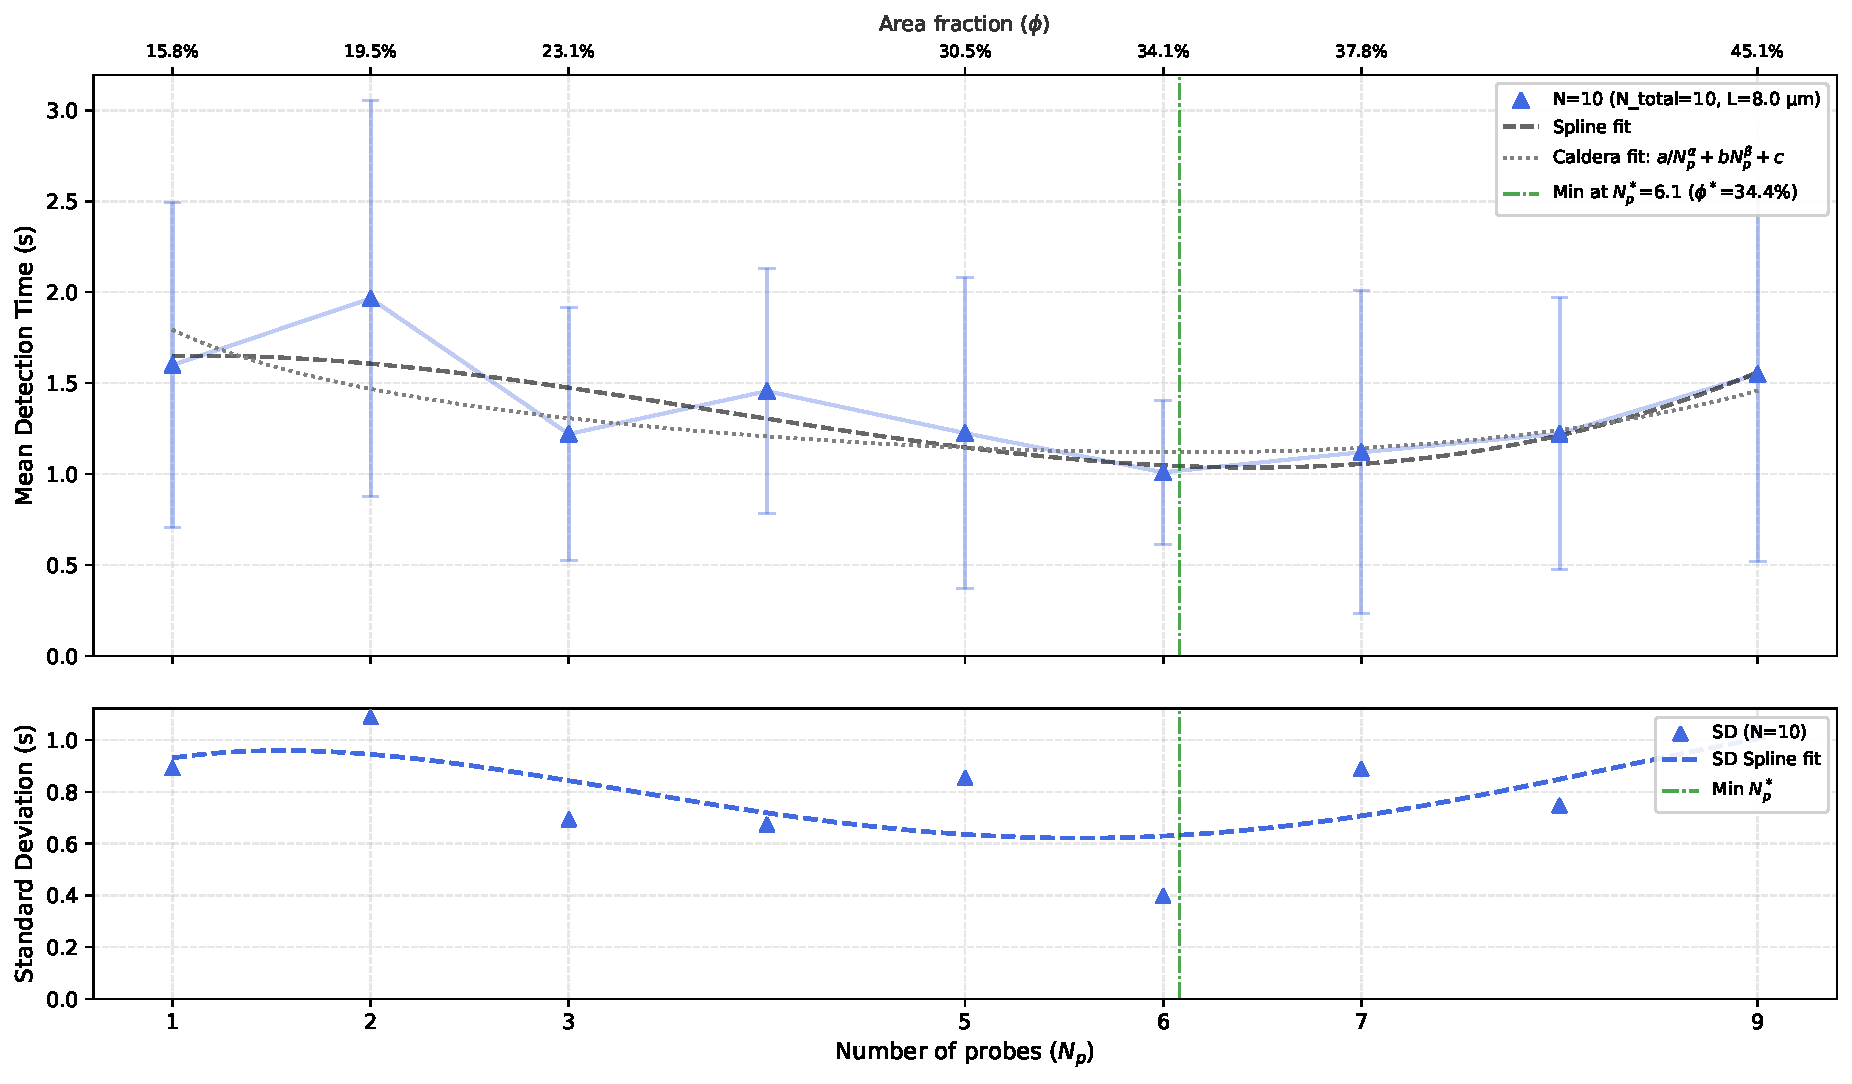
\includegraphics[width = 0.95\linewidth]{figures/caldera_individual_N_10.pdf}
    \caption{Mean first-passage detection time $\langle T \rangle$ (top) and its standard deviation (bottom) as a function of probe number $N_p$ (bottom axis) and area fraction $\phi$ (top axis) for the $N_\text{total} = 10$ system ($L = $ \SI{8.0}{\micro \meter}). The dotted curve is the caldera fit of Equation \ref{eq:3.6}; the dashed curve is the descriptive spline; the vertical dash-dot line marks the fitted optimum, $N_p = 6.1$ ($\phi \approx$ \SI{34.4}{\percent}).}
    \label{fig:Caldera10}
\end{figure}

\textbf{Figure~\ref{fig:Caldera10}} ($N_\text{total} = 10$) shows nine discrete probe counts available ($N_p = 1$ through $N_p = 9$), this is the coarsest-sampled system in the sweep, and it shows the noisiest curve of the six where its $\langle T \rangle$ rises from $N_p = 1$ to a local peak at $N_p = 2$ before beginning its overall decline, a non-monotonicity not seen in any larger system and consistent with run-to-run scatter dominating the signal at this system size. The minimum sits in a shallow, broad caldera spanning roughly $N_p = 5$--7 ($\phi \approx 30$--38\%), where the caldera fit and the descriptive spline agree closely, before both curves turn upward toward $N_p = 9$. The standard-deviation panel echoes this shape, narrowing to its tightest point near the fitted optimum and widening sharply at both the $N_p = 2$ and $N_p = 9$ extremes, with error bars at every point large enough to overlap several neighboring $N_p$ values.

\begin{figure}[htbp]
    \centering
    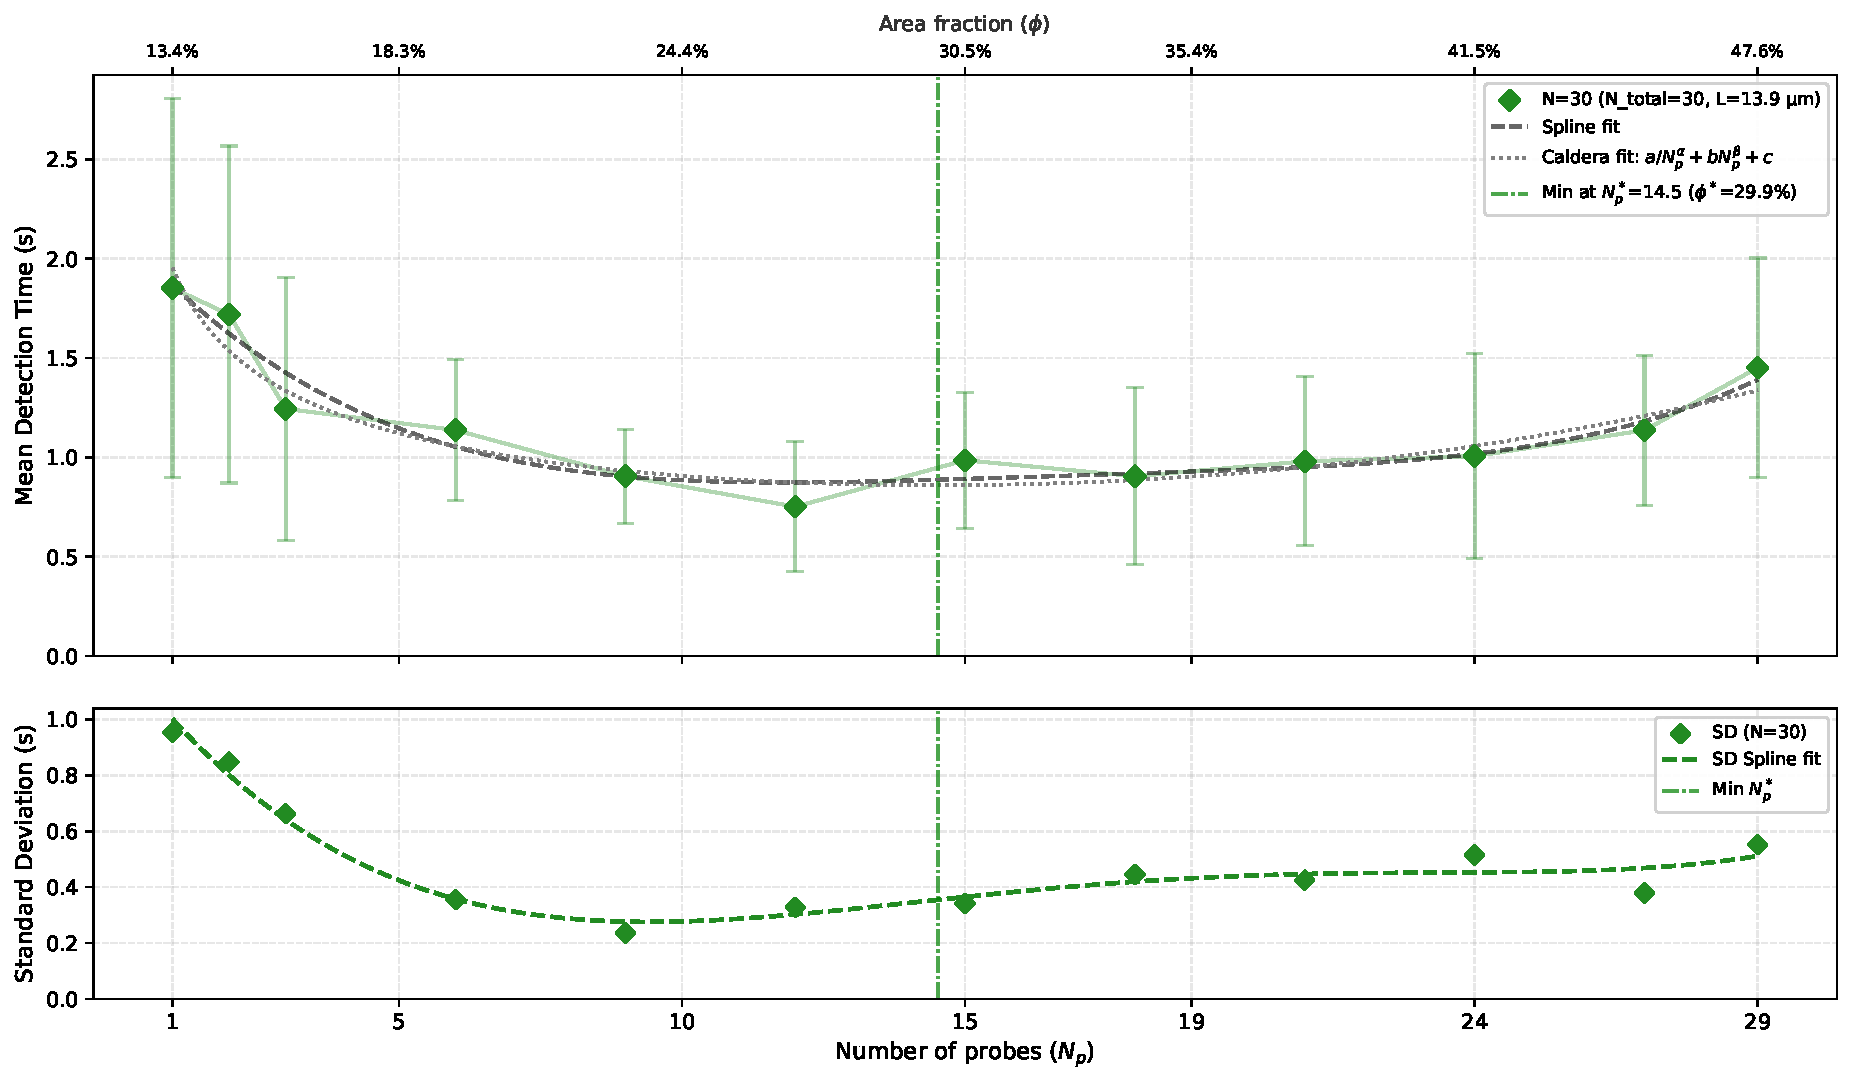
\includegraphics[width = 0.95\linewidth]{figures/caldera_individual_N_30.pdf}
    \caption{Mean first-passage detection time $\langle T \rangle$ (top) and its standard deviation (bottom) as a function of probe number $N_p$ (bottom axis) and area fraction $\phi$ (top axis) for the $N_\text{total} = 30$ system ($L = $ \SI{13.9}{\micro \meter}). The dotted curve is the caldera fit of Equation \ref{eq:3.6}; the dashed curve is the descriptive spline; the vertical dash-dot line marks the fitted optimum, $N_p = 14.5$ ($\phi \approx$ \SI{29.9}{\percent}).}
    \label{fig:Caldera30}
\end{figure}

\textbf{Figure~\ref{fig:Caldera30}} ($N_\text{total} = 30$) shows twelve sampled $N_p$ values, this curve is visibly smoother than the $N_\text{total} = 10$ case where its $\langle T \rangle$ falls steadily from its highest value at $N_p = 1$ to a floor spanning roughly $N_p = 9$--15 ($\phi \approx 23$--30\%), then rises gently but steadily out to $N_p = 29$. The caldera fit and the spline lie almost on top of one another across the entire sampled range, and the error bars while still substantial at $N_p = 1$--2, contract markedly once $N_p$ exceeds about 5. The standard-deviation panel reaches its minimum in the same $N_p$ window as $\langle T \rangle$'s floor and then climbs slowly and almost linearly through the rest of the sweep, without the sharp late upturn seen in the larger system below.

\begin{figure}[htbp]
    \centering
    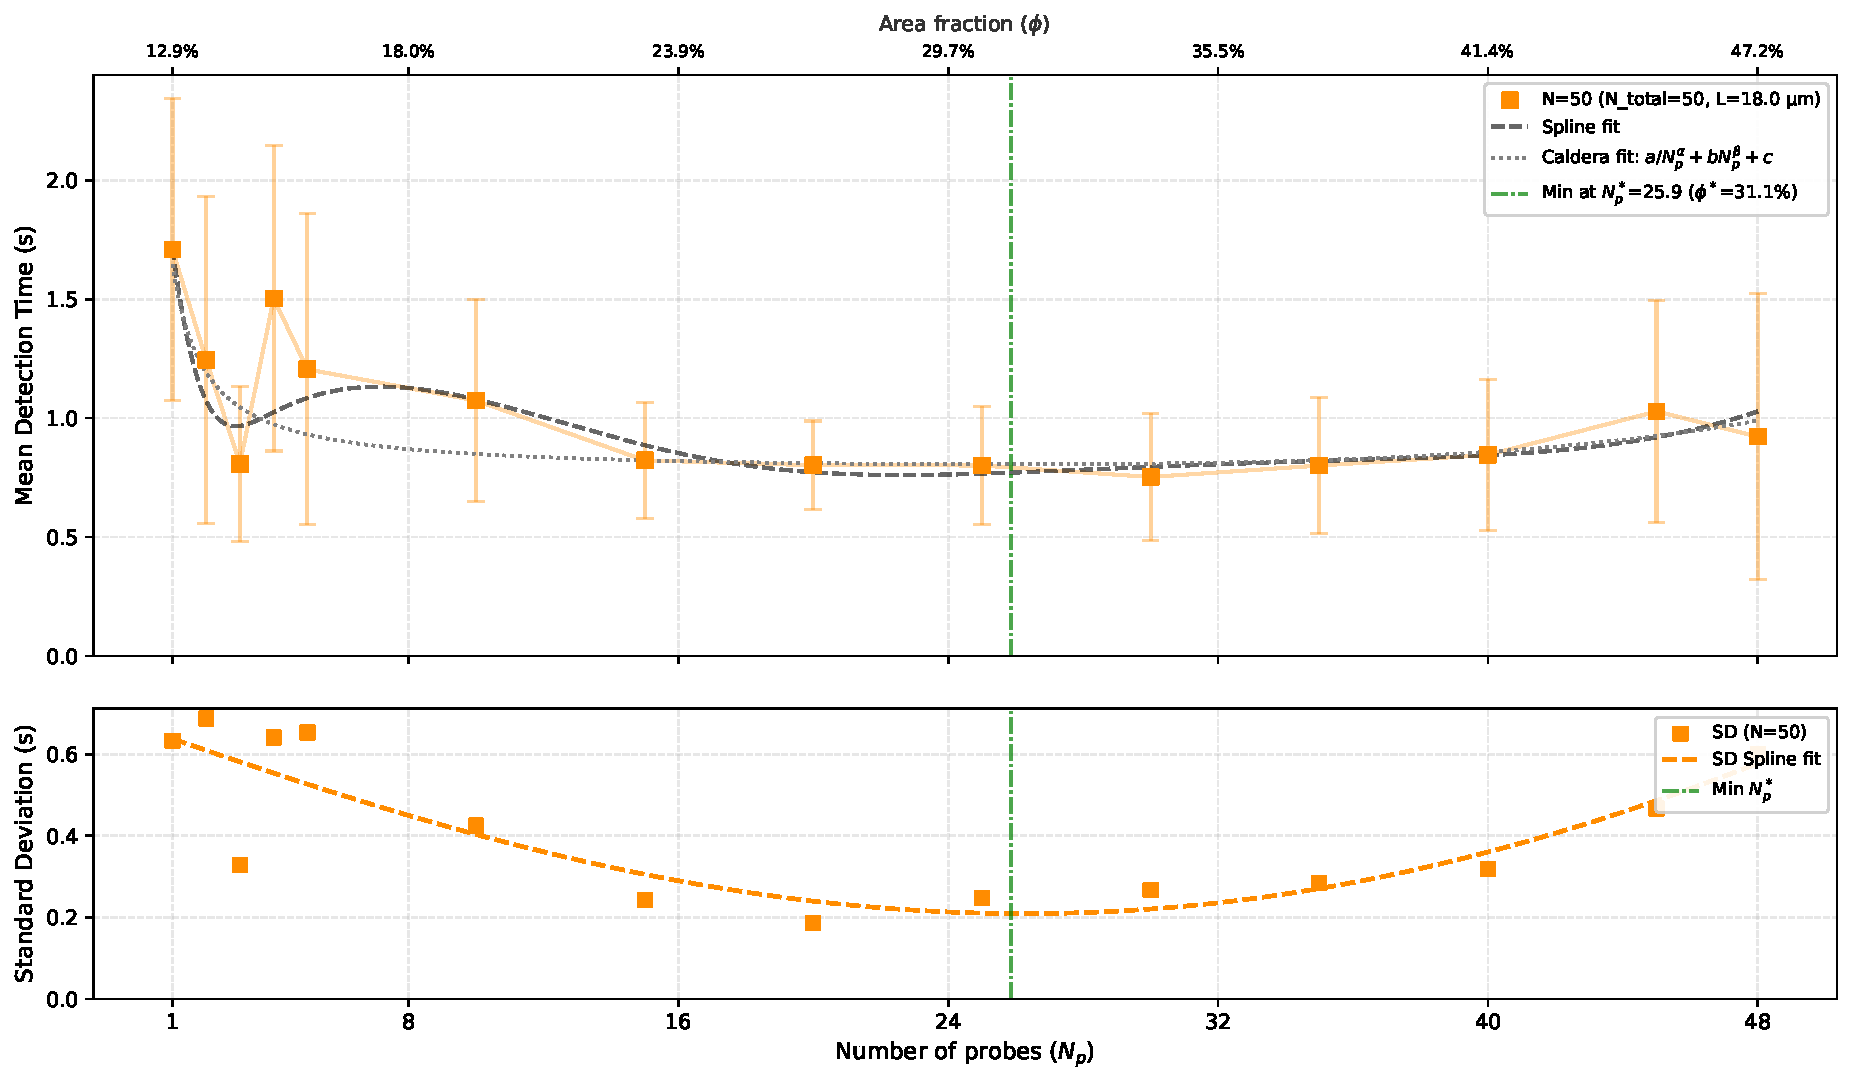
\includegraphics[width = 0.95\linewidth]{figures/caldera_individual_N_50.pdf}
    \caption{Mean first-passage detection time $\langle T \rangle$ (top) and its standard deviation (bottom) as a function of probe number $N_p$ (bottom axis) and area fraction $\phi$ (top axis) for the $N_\text{total} = 50$ system ($L = $ \SI{18.0}{\micro \meter}). The dotted curve is the caldera fit of Equation \ref{eq:3.6}; the dashed curve is the descriptive spline; the vertical dash-dot line marks the fitted optimum, $N_p = 25.9$ ($\phi \approx$ \SI{31.1}{\percent}).}
    \label{fig:Caldera50}
\end{figure}

\textbf{Figure~\ref{fig:Caldera50}} ($N_\text{total} = 50$) shows a pronounced early spike where its $\langle T \rangle$ at $N_p = 4$ briefly exceeds the values at $N_p = 2$, a small non-monotonicity similar in character (though milder than) the one seen at $N_\text{total} = 10$, before the curve settles into a long, flat floor extending from roughly $N_p = 16$ to $N_p = 32$ ($\phi \approx 24$--35\%). The caldera fit tracks the spline closely through this flat region and diverges only mildly on the crowded side, where the fit rises somewhat more gently than the raw points suggest. The standard deviation is largest and most erratic over the first few, most dilute points, drops to its lowest and most stable values across the same flat floor as $\langle T \rangle$, and turns upward again past $N_p \approx 32$, though this rise is modest compared to the sharper upturn seen in the three largest systems.

\begin{figure}[htbp]
    \centering
    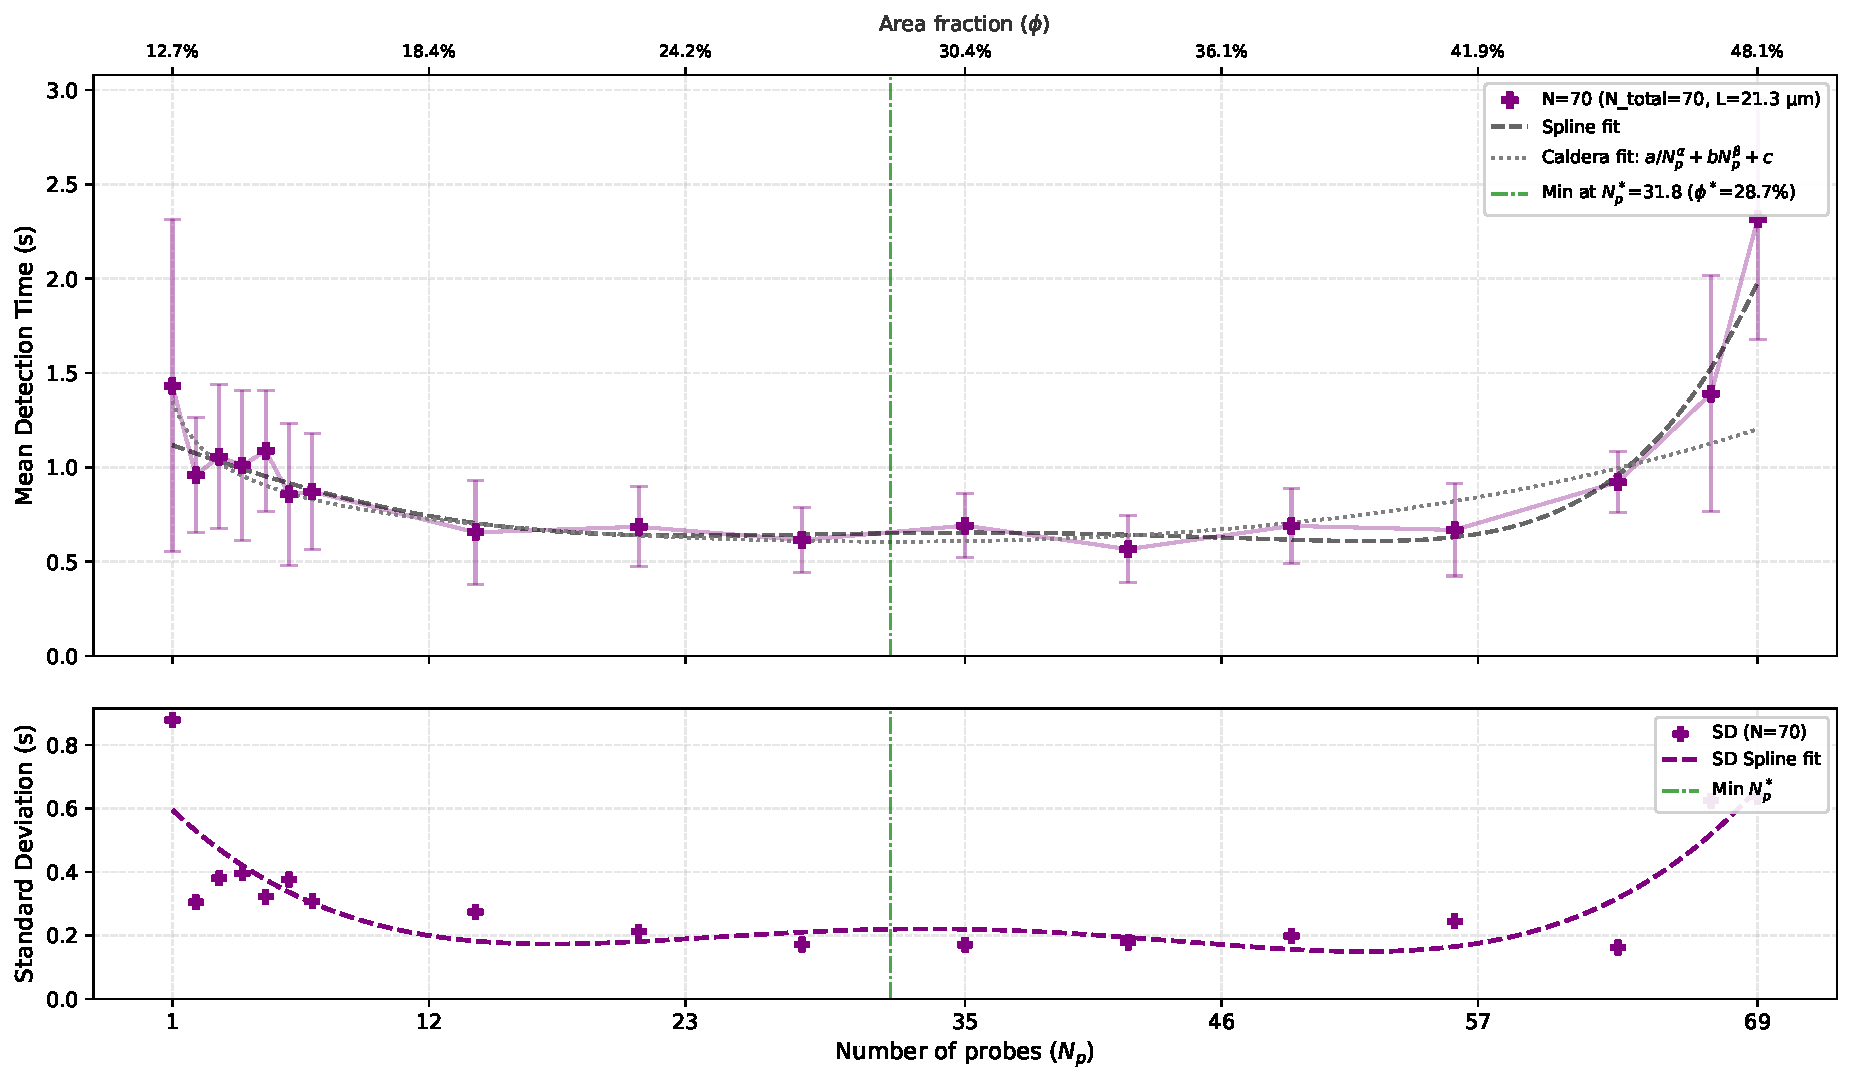
\includegraphics[width = 0.95\linewidth]{figures/caldera_individual_N_70.pdf}
    \caption{Mean first-passage detection time $\langle T \rangle$ (top) and its standard deviation (bottom) as a function of probe number $N_p$ (bottom axis) and area fraction $\phi$ (top axis) for the $N_\text{total} = 70$ system ($L = $ \SI{21.3}{\micro \meter}). The dotted curve is the caldera fit of Equation \ref{eq:3.6}; the dashed curve is the descriptive spline; the vertical dash-dot line marks the fitted optimum, $N_p = 31.8$ ($\phi \approx$ \SI{28.7}{\percent}).}
    \label{fig:Caldera70}
\end{figure}

\textbf{Figure~\ref{fig:Caldera70}} ($N_\text{total} = 70$) is the first system in the sweep where the caldera shape becomes visually ambiguous rather than merely fitted. Its $\langle T \rangle$ drops sharply over the first dozen or so probes, settles into a long, low, comparatively flat plateau from roughly $N_p = 12$ to $N_p =46$ ($\phi\approx 18$--42\%), and then rises sharply and clearly over the final several points, with the last two or three sampled conditions visibly separated from the plateau even accounting for their error bars. The standard deviation is lowest and most tightly clustered across the same wide plateau and increases sharply in step with $\langle T \rangle$ at the crowded edge, more than doubling between the floor and the final sampled point. This is the first system size at which the crowded-side rise is clearly resolved above the noise floor rather than merely suggested by the fit.

\begin{figure}[H]
    \centering
    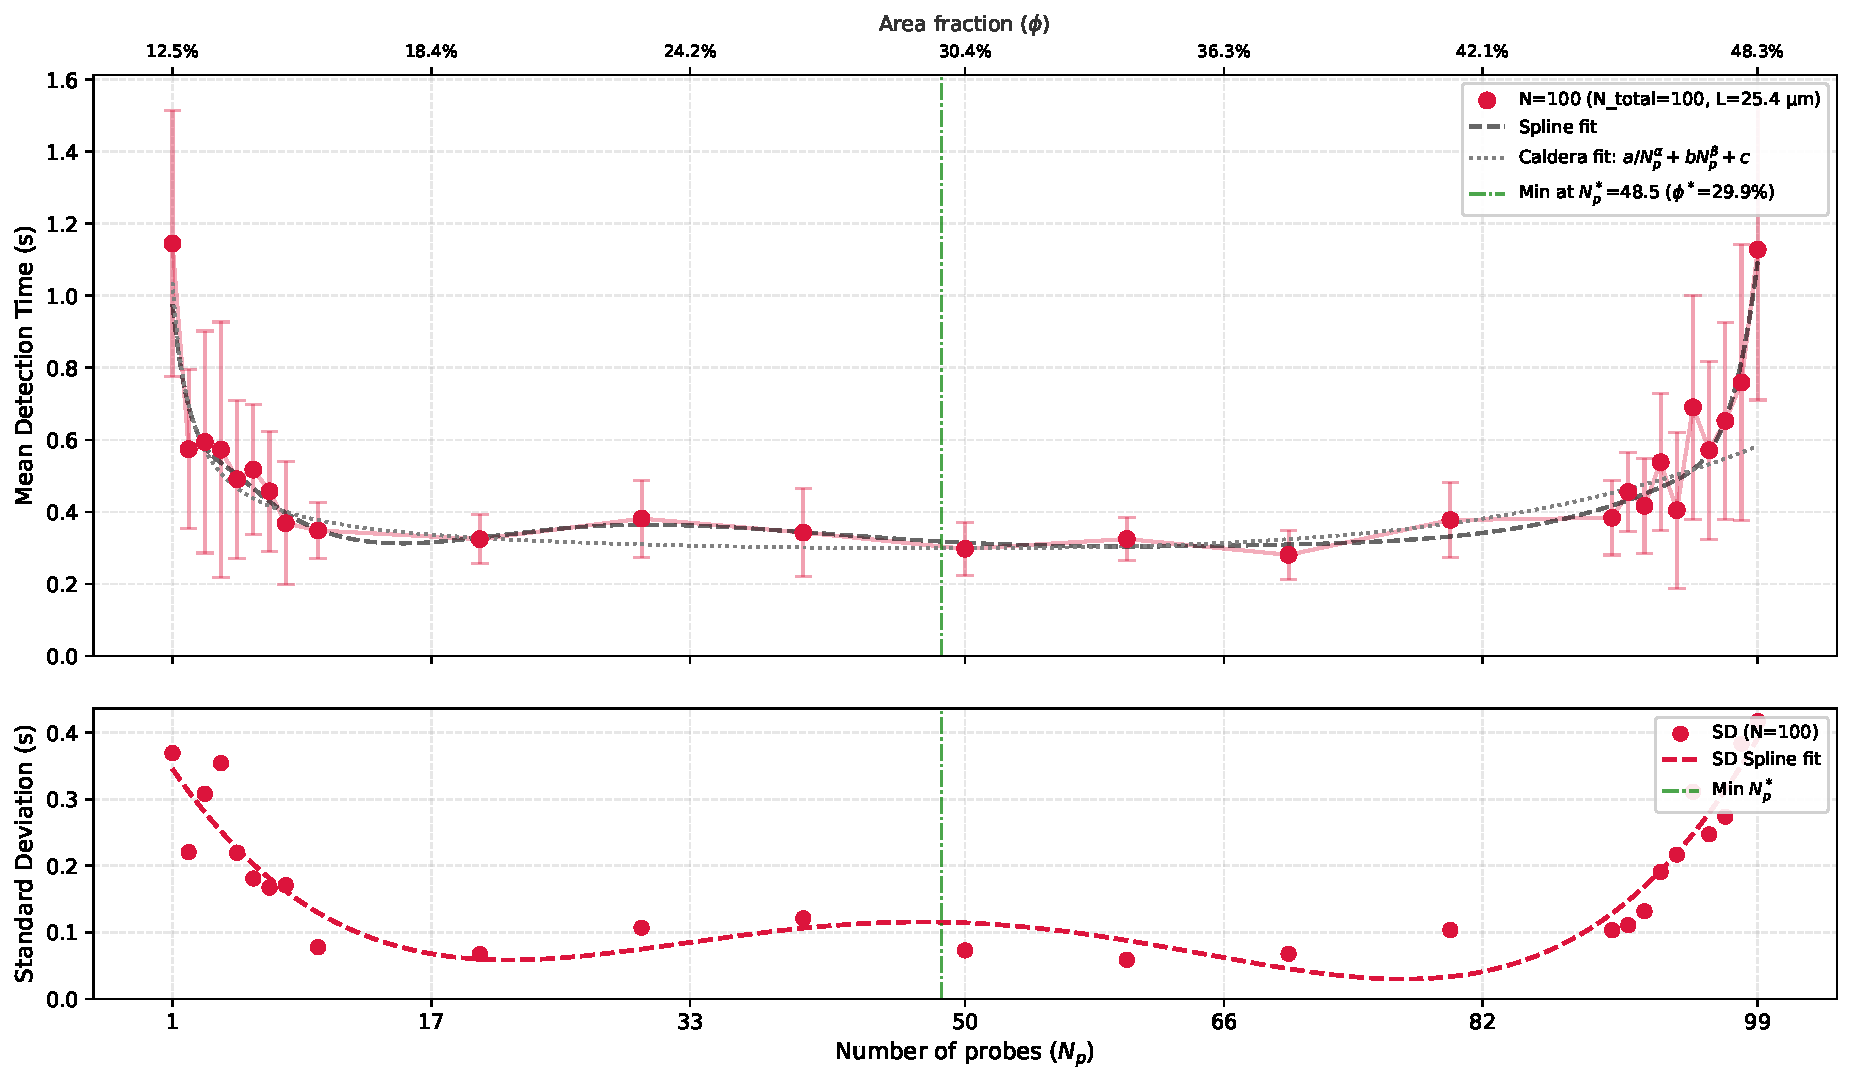
\includegraphics[width = 0.95\linewidth]{figures/caldera_individual_N_100.pdf}
    \caption{Mean first-passage detection time $\langle T \rangle$ (top) and its standard deviation (bottom) as a function of probe number $N_p$ (bottom axis) and area fraction $\phi$ (top axis) for the $N_\text{total} = 100$ system ($L = $ \SI{25.4}{\micro \meter}). The dotted curve is the caldera fit of Equation \ref{eq:3.6}; the dashed curve is the descriptive spline; the vertical dash-dot line marks the fitted optimum, $N_p = 48.5$ ($\phi \approx$ \SI{29.9}{\percent}).}
    \label{fig:Caldera100}
\end{figure}

\textbf{Figure~\ref{fig:Caldera100}} ($N_\text{total} = 100$) shows twenty sampled $N_p$ values, and this is one of the two most finely resolved systems in the sweep, and its caldera shape is the cleanest of the six. Its $\langle T \rangle$ falls from just over 1\,s at $N_p=1$ to a floor near 0.3\,s that is sustained, essentially flat, from roughly $N_p =17$ to $N_p = 66$ ($\phi \approx 18$--36\%), before rising steeply over the last quarter of the sweep to end close to its starting value near $N_p = 99$. The standard deviation mirrors this shape almost exactly, falling 0.1\,s across the plateau and climbing back above 0.3\,s at the crowded edge. The caldera fit and spline are nearly indistinguishable thorugh the plateau and separate only slightly on the crowded flank, where the raw points show somewhat more scatter than the smooth fit implies.

\begin{figure}[H]
    \centering
    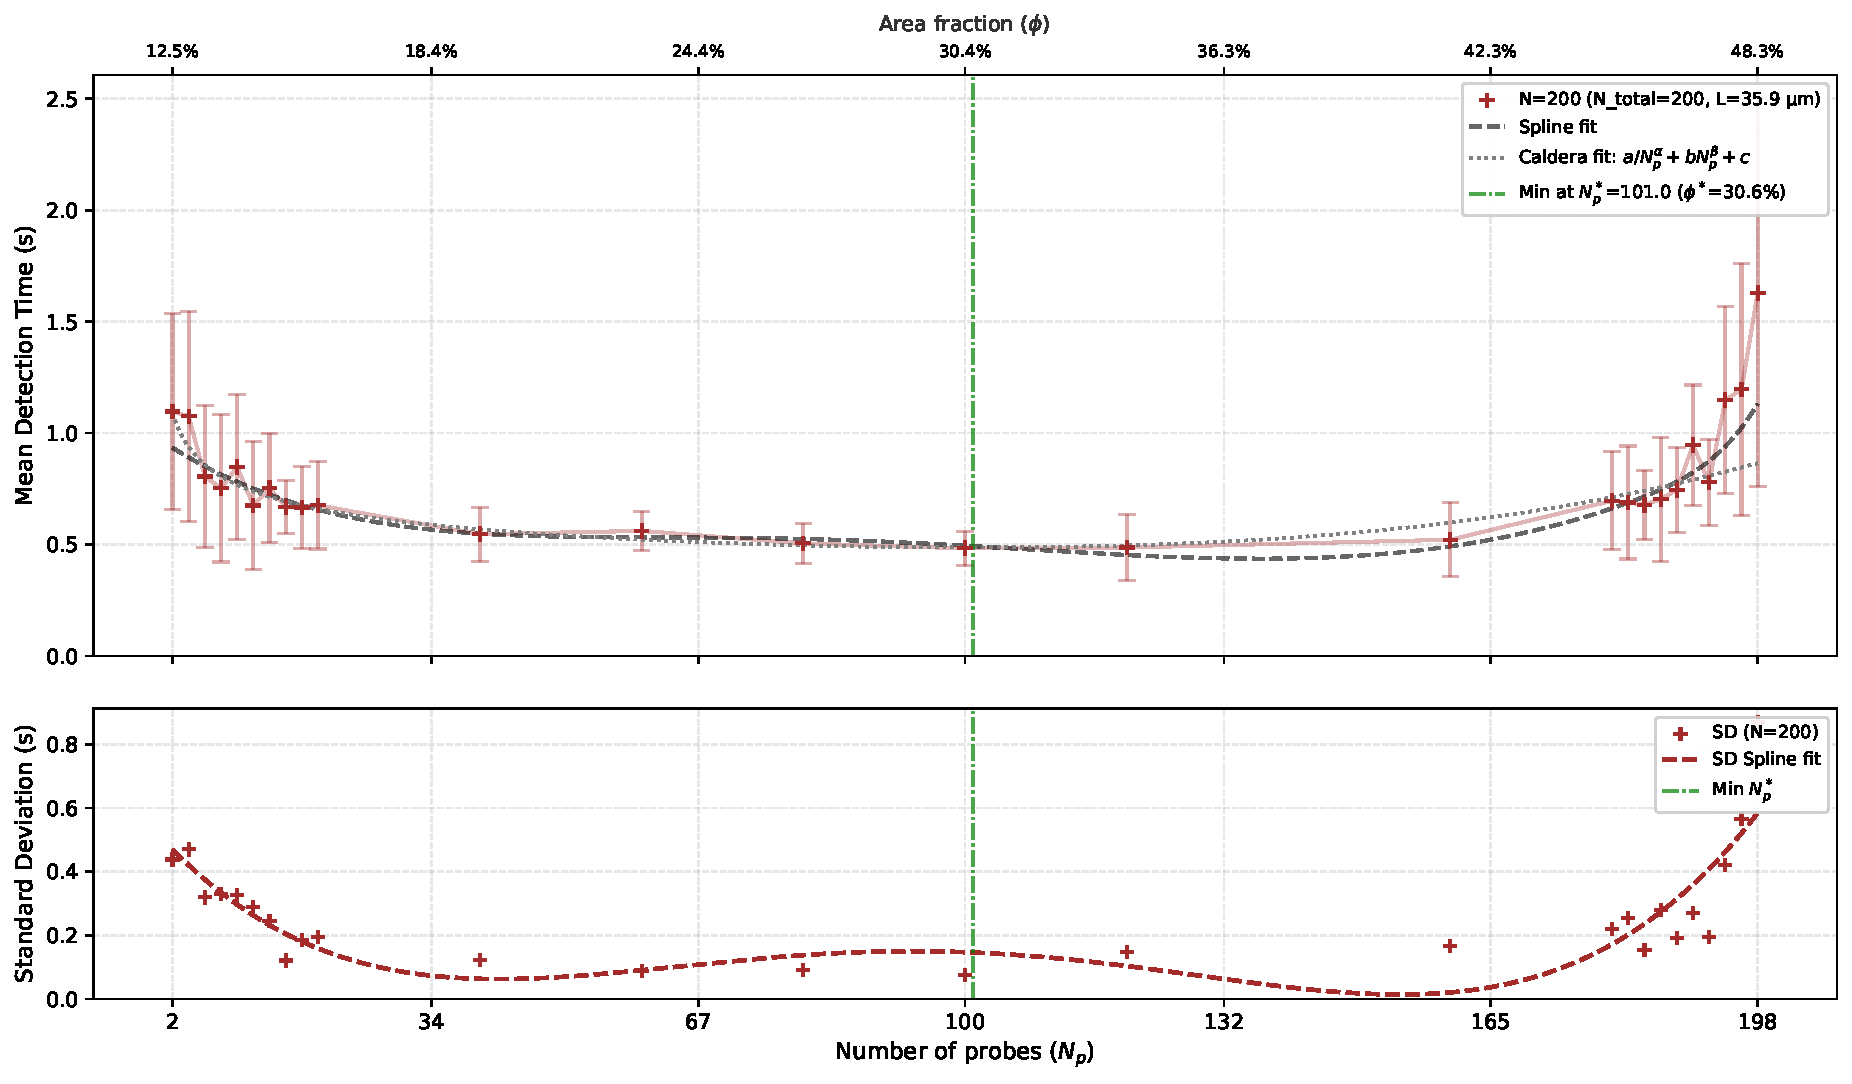
\includegraphics[width = 0.95\linewidth]{figures/caldera_individual_N_200.pdf}
    \caption{Mean first-passage detection time $\langle T \rangle$ (top) and its standard deviation (bottom) as a function of probe number $N_p$ (bottom axis) and area fraction $\phi$ (top axis) for the $N_\text{total} = 200$ system ($L = $ \SI{35.9}{\micro \meter}). The dotted curve is the caldera fit of Equation \ref{eq:3.6}; the dashed curve is the descriptive spline; the vertical dash-dot line marks the fitted optimum, $N_p = 101.0$ ($\phi \approx$ \SI{30.6}{\percent}).}
    \label{fig:Caldera200}
\end{figure}

\textbf{Figure~\ref{fig:Caldera200}} ($N_\text{total} = 200$) shows the largest and most finely sampled system, this plot shows the widest and flattest floor of the six, extending from roughly $N_p = 34$ to $N_p = 132$ ($\phi \approx 18$--42\%) at a level near 0.5\,s which is noticeable higher than the $N_\text{total}=100$ floor, the reversal discussed in Section~\ref{sec:4.10}. The rise at the crowded edge is the steepest of any system in absolute terms, with the final few moments climbing past 1.5--2.5\,s and carrying the widest error bars in the entire sweep. The standard-deviation panel is correspondingly the most dramatic where it sits below 0.2\,s for the majority of the sampled range and rises sharply, almost vertically, over the last five or six points, indicating that both the typical detection time and its run-to-run variability degrade together once probe density passes roughly $\phi \approx 42$--48\%.

\section{Locating the Optimum: The Caldera Fit}
\label{sec:4.2}

Fitting equation~\ref{eq:3.6} to each system's $N_p, \langle T \rangle$ data locates a well-defined optimum in every case (Figures \ref{fig:Caldera10}--\ref{fig:Caldera200}, dotted curves). The fitted optimal probe number $N_p^*$ and corresponding area fraction $\phi^*$ for each system are summarized in Table~\ref{tab:caldera-optima}

% \begin{table}[htbp]
%     \centering
%     \caption{Fitted caldera optimum probe number and area fraction per system size.}
%     \begin{tabular}{ccc}
%     \hline   
%         $N_\text{total}$ & $N_p^*$ & $\phi^*$ \\
%     \hline     
%          10 & 6.1 & 34.4  \\
%          30 & 14.5 & 29.9  \\
%          50 & 25.9 & 31.1  \\
%          70 & 31.8 & 28.7  \\
%          100 & 48.5 & 29.9  \\
%          200 & 101.0 & 30.6  \\
%     \hline     
%     \end{tabular}
%     \label{tab:caldera-optima}
% \end{table}

\begin{table}[htbp]
\centering
\caption{Fitted caldera optimum probe number and area fraction per system size.}
\begin{tabular}{ccccccc}
\hline
\textbf{N$_\text{total}$} & \textbf{10} & \textbf{30} & \textbf{50} & \textbf{70} & \textbf{100} & \textbf{200} \\ \hline
\textbf{$N^*_p$}          & 6.1         & 14.5        & 25.9        & 31.8        & 48.5         & 101.0        \\
\textbf{$\phi^*$}         & 34.4        & 29.9        & 31.1        & 28.7        & 29.9         & 30.6         \\ \hline
\end{tabular}
\label{tab:caldera-optima}
\end{table}

Excluding $N_\text{total} = 10$, the fitted $\phi^*$ clusters tightly between 28.7\% and 31.1\% with a mean of $\approx 30.1\%$ despite the tenfold range in absolute system size from $N_\text{total} = 30$ to 200. The $N_\text{total} = 10$ system is a mild outlier at $\phi^* = 34.4\%$, a departure addressed directly in Section~\ref{sec:4.7}. In every system, the caldera fit (dotted) and the descriptive spline (dashed) track each other closely near the minimum, with the closest agreement in the $N_\text{total} = 30$, 50, 70, and 100 systems and the widest separation in the $N_\text{total} = 10$ system, where only nine discrete $N_p$ values are available to constrain the fit. Read together with the per-figure descriptions above, the fitted optimum consistently lands inside each system's visually flattest region of $\langle T \rangle$ rather than at an isolated point, which is the qualitative check that the two-term model of Equation~\ref{eq:3.6} is capturing a genuine caldera rather than over-fitting to a single low-noise data point.

\begin{figure}[htbp]
    \centering
    \includegraphics[width = 0.95\linewidth]{figures/Fig5_floor_summary.pdf}
    \caption{Floor-vs-system detection of mean detection time $\langle T \rangle$ and the Standard deviation time plotted against all the system size showing non-monotonic relationship of minimum detection with system size.}
    \label{fig:floorvssystem}
\end{figure}

Having identified the floor detection time for each system, Figure~\ref{fig:floorvssystem} compares these floor values directly across system sizes. The top panel shows the floor mean detection time $\langle T \rangle$, and the bottom panel shows its associated standard deviation, both plotted against $N_\text{total}$. The floor value decreases from $N=10$ through $N=100$, but then rises again at $N=200$, which indicates that the floor detection time is non-monotonic with system size rather than continuing to improve as the system grows. This suggests that increasing the overall system size does not uniformly improve the best achievable detection time once probe density is already optimized; beyond a certain scale (here, between $N=100$ and $N=200$), enlarging the system appears to work against detection efficiency at the floor, even though the same range of area fractions is sampled in both cases. A plausible explanation is that fixing the area fraction across differently sized systems does not fix the absolute length scales of the search domain which means a larger box at the same $\phi$ still requires probes and targets to cover proportionally larger physical distances between collisions, which can offset the benefit of having more probes available. The standard deviation panel shows the same qualitative trend, with the lowest run-to-run variability also occurring near $N=100$, suggesting this system size sits closest to an overall efficient and consistent detection regime within the range studied.

\section{Variance and Reliability Across the Search}
\label{sec:4.3}

\begin{figure}[htbp]
    \centering
    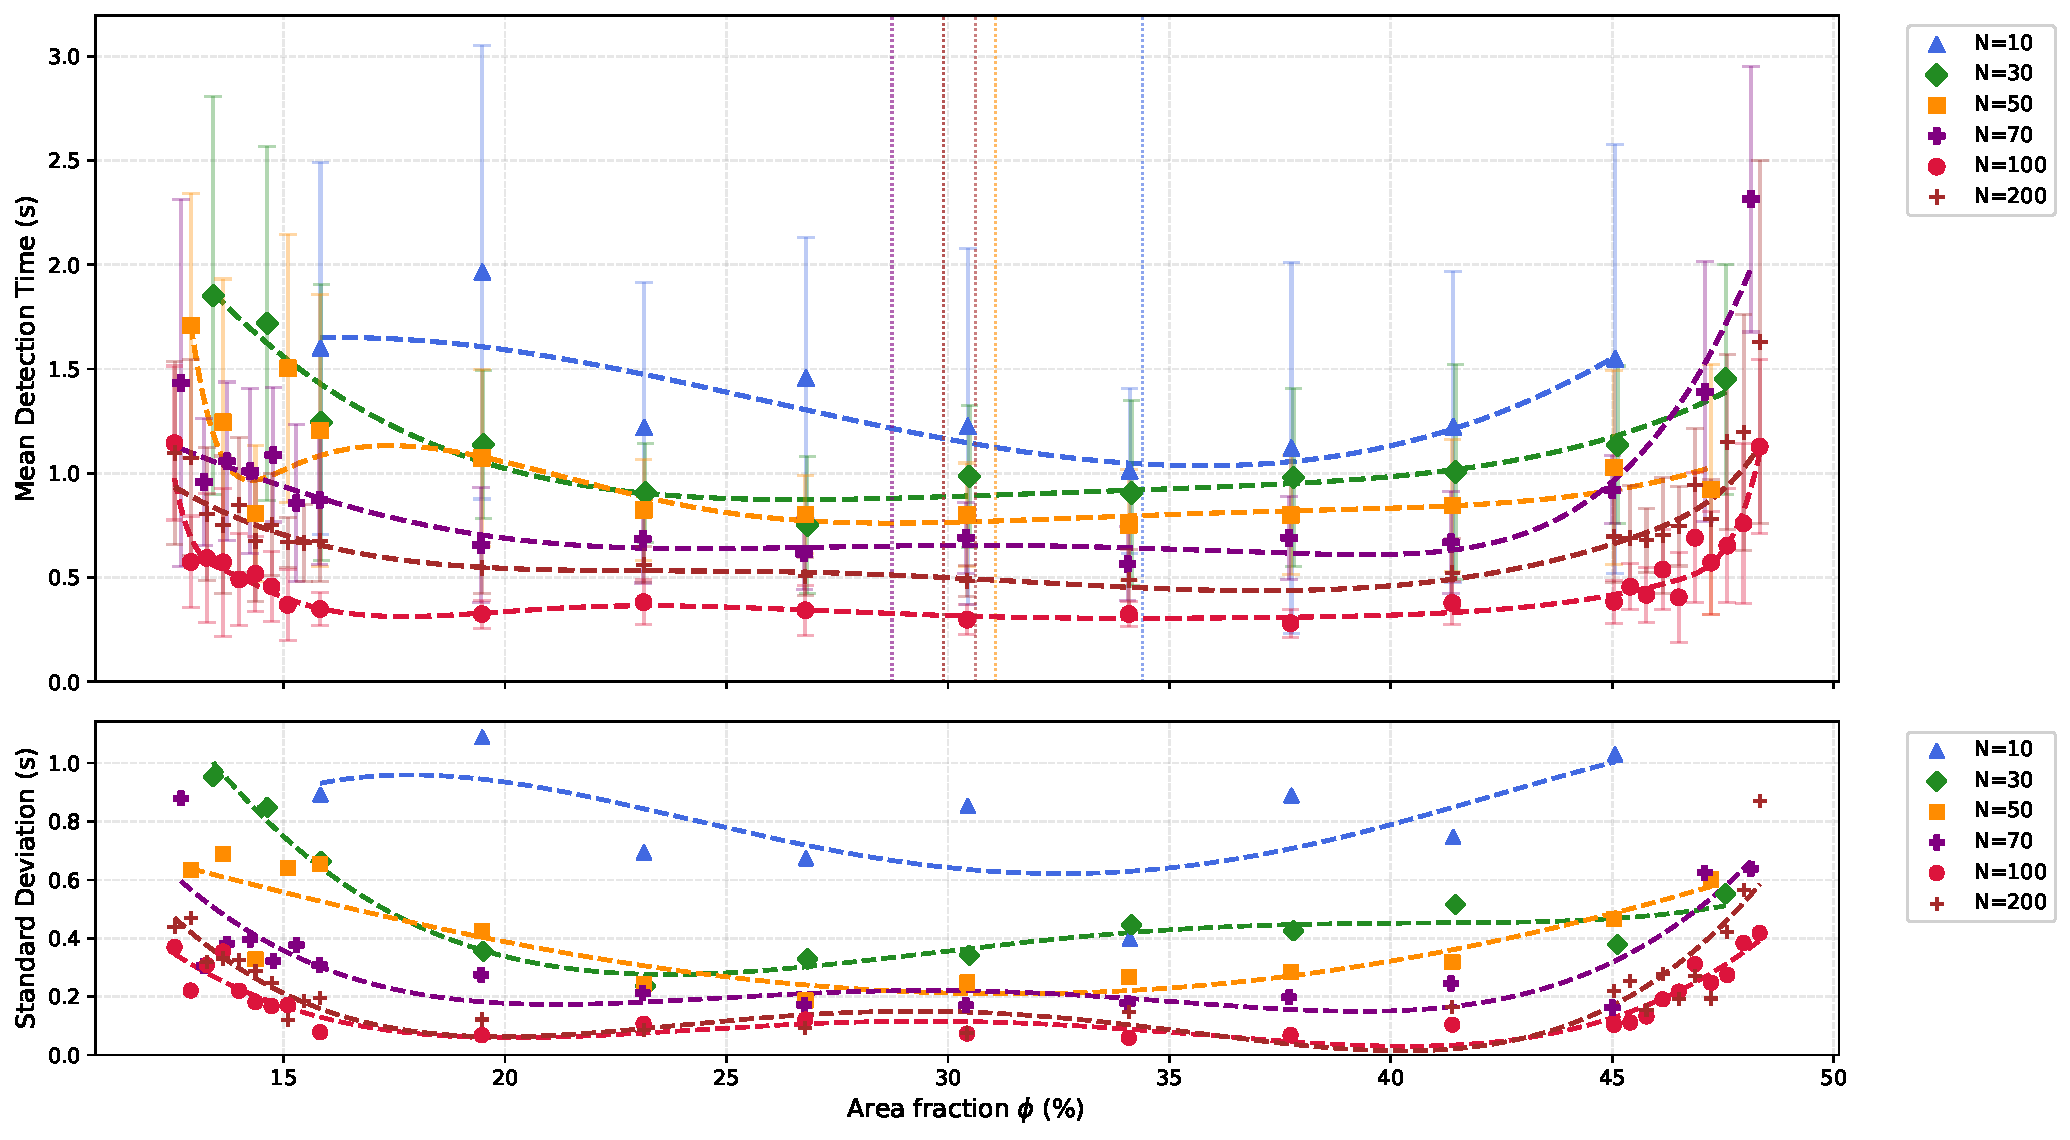
\includegraphics[width = 0.95\linewidth]{figures/caldera_overlay_phi.pdf}
    \caption{Overlay of mean first-passage detection time (top) and standard deviation (bottom) versus area fraction $\phi$ for all six system sizes ($N_\text{total} = 10,30,50,70, 100,200$), each with its own descriptive spline fit, allowing the caldera minimum and the width of the crowding onset to be compared directly across system scales on a common $\phi$ axis.}
    \label{fig:OverlayCaldera}
\end{figure}

\textbf{Figure~\ref{fig:OverlayCaldera}} plots all six systems on a common area-fraction axis, rather than on their individual $N_P$ axes, makes two features visible that are hard to see in Figures~\ref{fig:4.1}--\ref{fig:4.6} taken one at a time. First, the six curves are stacked in the same order in both panels throughout the sampled range. $N_\text{total} = 10$ sits highest in both $\langle T \rangle$ and standard deviation at almost every $\phi$, while $N_\text{total} =100$ sits lowest, with $N_\text{total} =200$ tucked just above it rather than below it, reproducing the floor-value reversal noted in Section~\ref{sec:4.1}. Second, the minima of all six splines cluseter in a visibly narrow band of the shared $\phi$ axis, roughly between 25\% and 35\%, even though the curves are otherwise offset from one another by as much as a factor of two to three in absolute $\langle T \rangle$. The overlay overlay shows that the same caldera structure seen in $\langle T \rangle$ appears independently in the standard deviation, for every system size where this is a non-trivial consistency check, since it means the caldera minimum in $\langle T \rangle$ is not merely a shift in central tendency accompanied by unchanged or worsening spread, this means that the search becomes both faster and more reproducible across independent seeds in the same $N_p$/$\phi$ window. Across the larger systems ($N_\text{total} = 70, 100, 200$), the standard deviation rises more steeply on the crowded (high-$N_p$) side of the caldera than it falls on the dilute side; for example, in the $N_\text{total} = 100$ system the standard deviation grows from roughly 0.1\,s near the floor to over 0.3\,s by $N_p =99$, a threefold increase, while the corresponding rise in $\langle T \rangle$ over the same range is comparatively more gradual. This asymmetric growth in variance, ahead of a comparably sharp rise in the mean, foreshadows the distributional broadening examined directly in Section~\ref{sec:4.5}.

\section{The Ergodic Product}
\label{sec:4.4}

The ergodic product $E = N_p \times \langle T \rangle$ tracks its linear sub-critical extrapolation closely at low $N_p$ in every system, by construction, and departs upward from that extrapolation as $N_p$ increases. The six individual plots  (Figures~\ref{fig:ErgodicProduct10}--\ref{fig:ErgodicProduct200}) and their cross-system overlay (Figure~\ref{fig:OverlayErgodicProduct}) are described in turn below.

\begin{figure}[htbp]
    \centering
    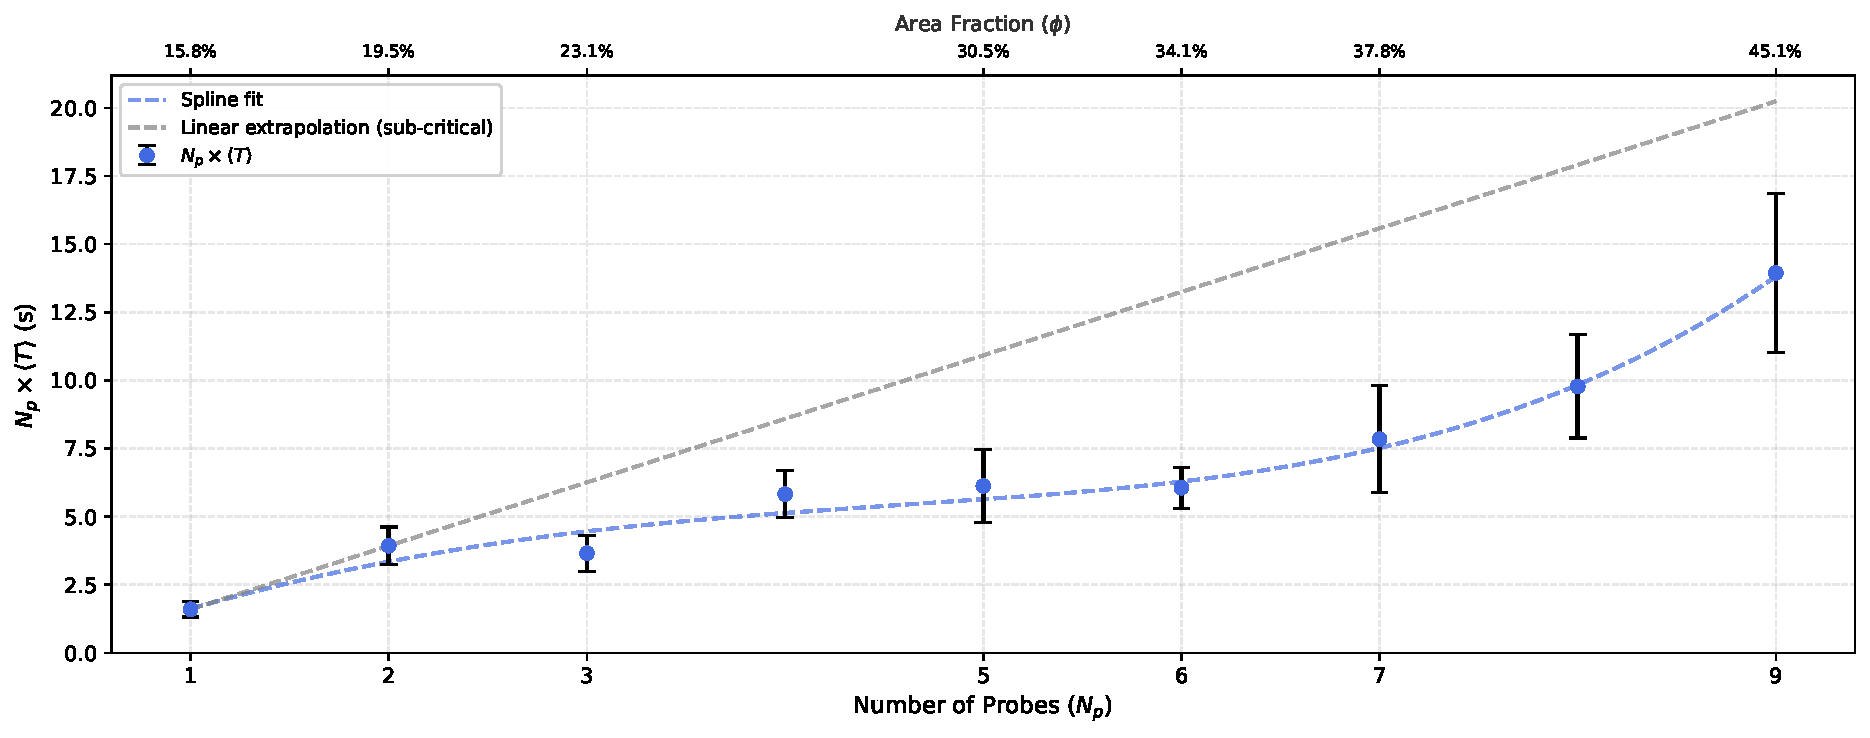
\includegraphics[width = 0.95\linewidth]{figures/ergodic_individual_N_10.pdf}
    \caption{Ergodic product $E = N_p\times \langle T\rangle$ versus $N_p$ and $\phi$ for the $N_\text{total} = 10$ system. The dashed line is a linear extrapolation of $E$ from the most dilute (sub-critical) points, representing the ideal, non-interacting-searcher expectation; the spline traces the actual measured values, and its upward departure from the extrapolation signals the onset of non-ergodic, crowding-influenced search.}
    \label{fig:ErgodicProduct10}
\end{figure}

\textbf{Figure~\ref{fig:ErgodicProduct10}} ($N_\text{total} = 10$) shows that $E$ tracks its sub-critical extrapolation reasonably well through the first four or five probe counts, but the departure that follows is gradual rather than sharp, and the error bars which are already wide in absolute $\langle T \rangle$ for this system (Figure~\ref{fig:Caldera10}) grows wide enough by $N_p = 7$--9 to overlap the extrapolation line itself. A departure is visually suggested by $N_p = 7$, but it cannot be called unambiguous given the size of the uncertainty at that point. 

\begin{figure}[htbp]
    \centering
    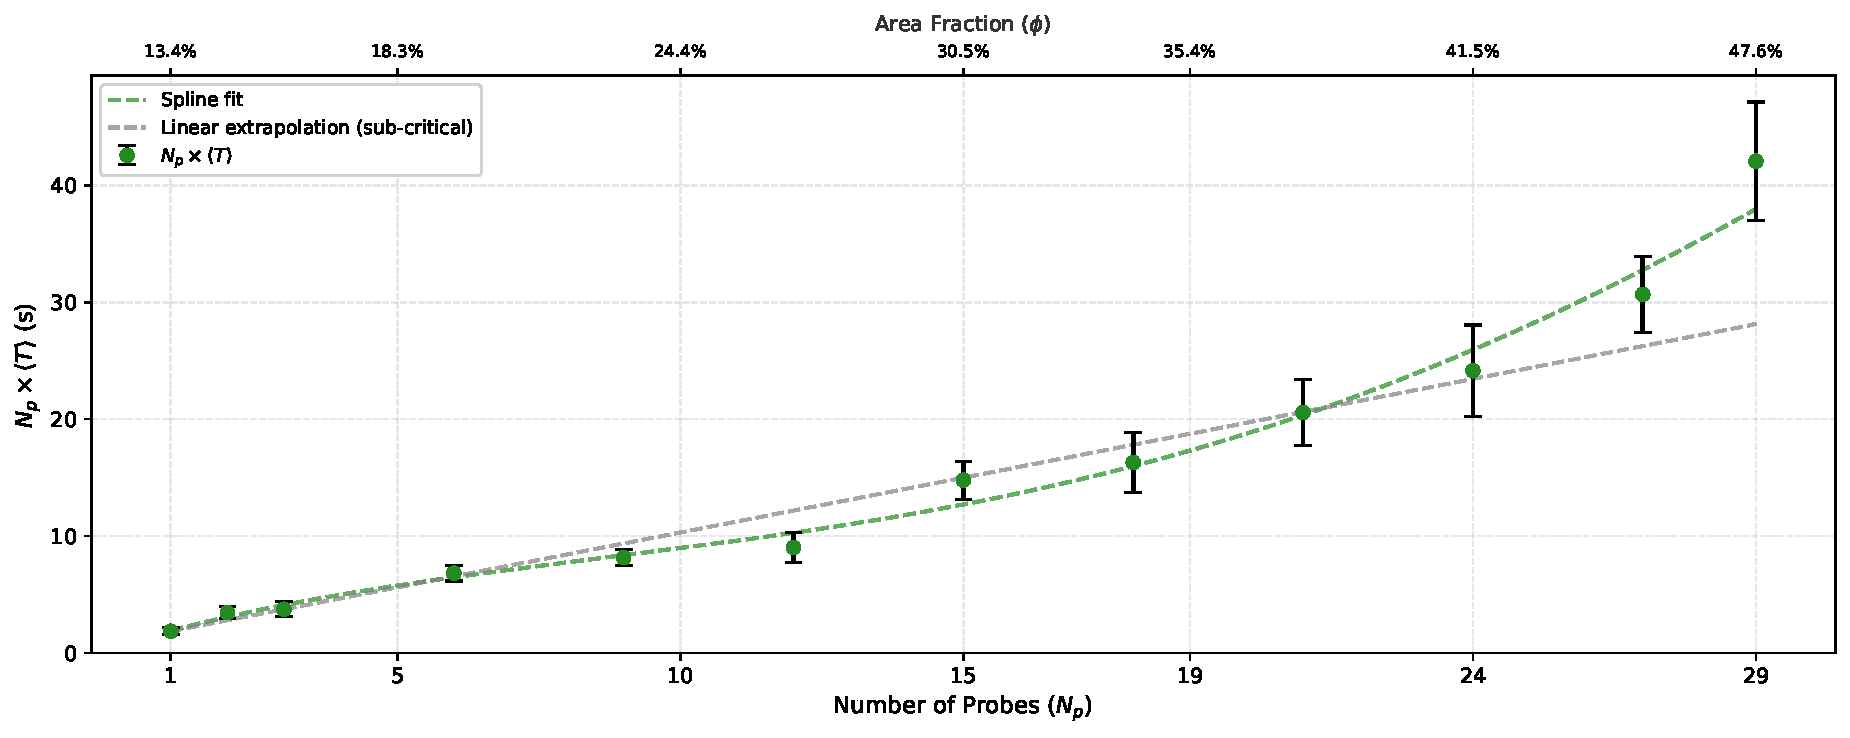
\includegraphics[width = 0.95\linewidth]{figures/ergodic_individual_N_30.pdf}
    \caption{Ergodic product $E = N_p\times \langle T\rangle$ versus $N_p$ and $\phi$ for the $N_\text{total} = 30$ system. The dashed line is a linear extrapolation of $E$ from the most dilute (sub-critical) points, representing the ideal, non-interacting-searcher expectation; the spline traces the actual measured values, and its upward departure from the extrapolation signals the onset of non-ergodic, crowding-influenced search.}
    \label{fig:ErgodicProduct30}
\end{figure}

\textbf{Figure~\ref{fig:ErgodicProduct30}} ($N_\text{total} = 30$) shows that $E$ follows its extrapolation closely and with tight error bars out to roughly $N_p = 19$, then separates visibly, if still gently, over the last three sampled points, reaching roughly 1.3--1.5$\times$ the extrapolated value by $N_\text{total} = 10$ system but remains modest in magnitude relative to the sharp separations seen in the larger systems below.

\begin{figure}[htbp]
    \centering
    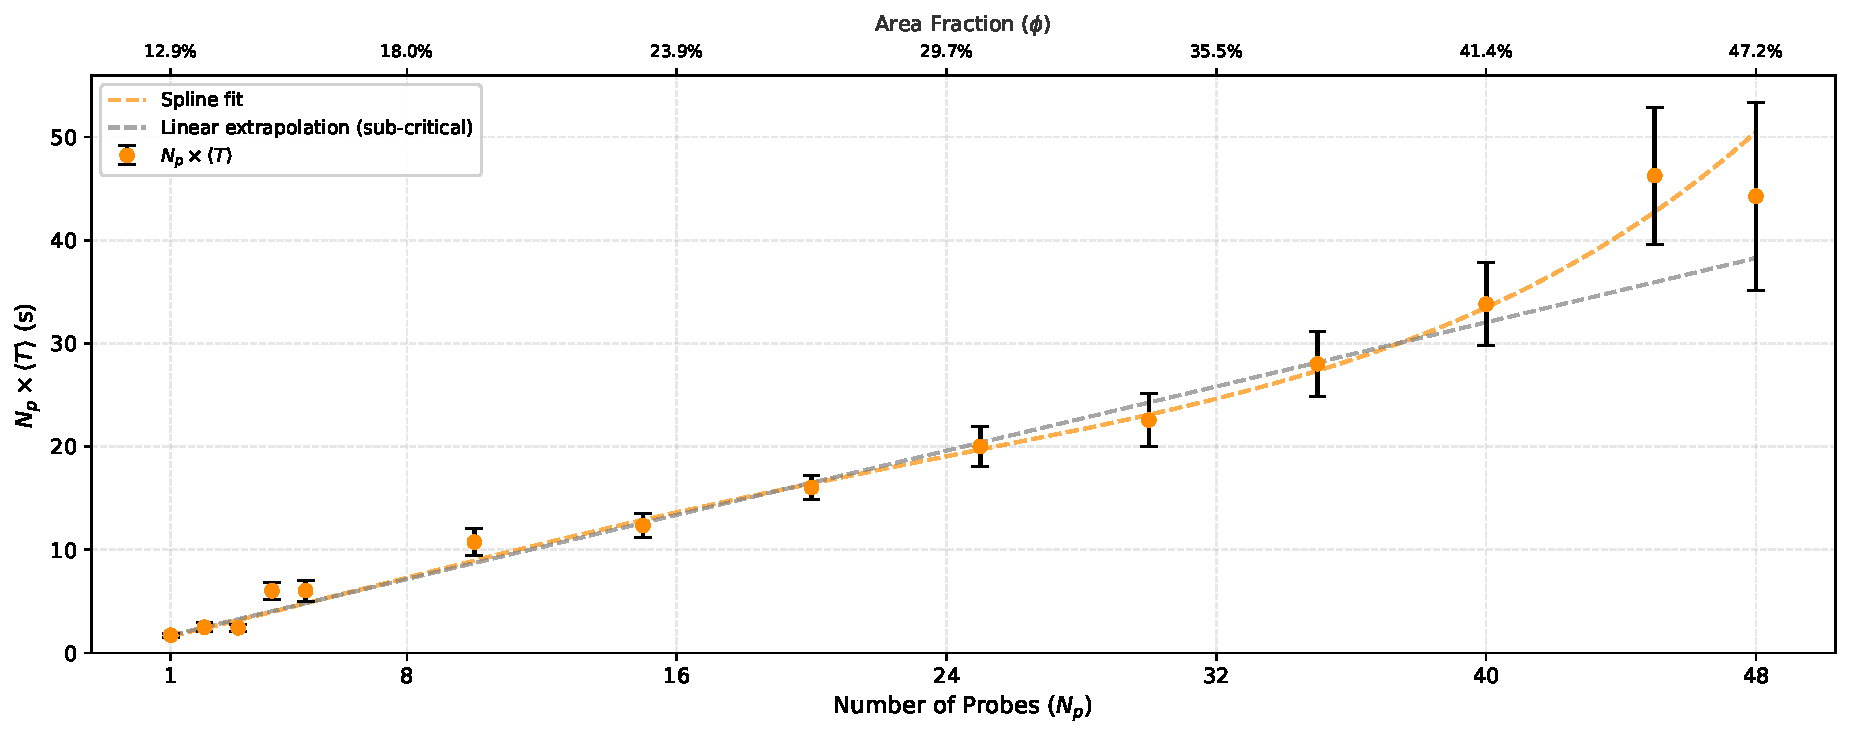
\includegraphics[width = 0.95\linewidth]{figures/ergodic_individual_N_50.pdf}
    \caption{Ergodic product $E = N_p\times \langle T\rangle$ versus $N_p$ and $\phi$ for the $N_\text{total} = 50$ system. The dashed line is a linear extrapolation of $E$ from the most dilute (sub-critical) points, representing the ideal, non-interacting-searcher expectation; the spline traces the actual measured values, and its upward departure from the extrapolation signals the onset of non-ergodic, crowding-influenced search.}
    \label{fig:ErgodicProduct50}
\end{figure}

\textbf{Figure~\ref{fig:ErgodicProduct50}} ($N_\text{total} = 50$) shows the measured $E$ and its extrapolation are nearly coincident through the first twenty-four probes, with small, tight error bars throughout this range. The departure appears only at the last two sampled points ($N_p =40$ and 48), where $E$ rises to roughly 1.3--1.5$\times$ the extrapolated values where the error bars at these two points are wider than elsewhere in the curve but still leave the departure visually distinguishable from the extrapolation line.

\begin{figure}[htbp]
    \centering
    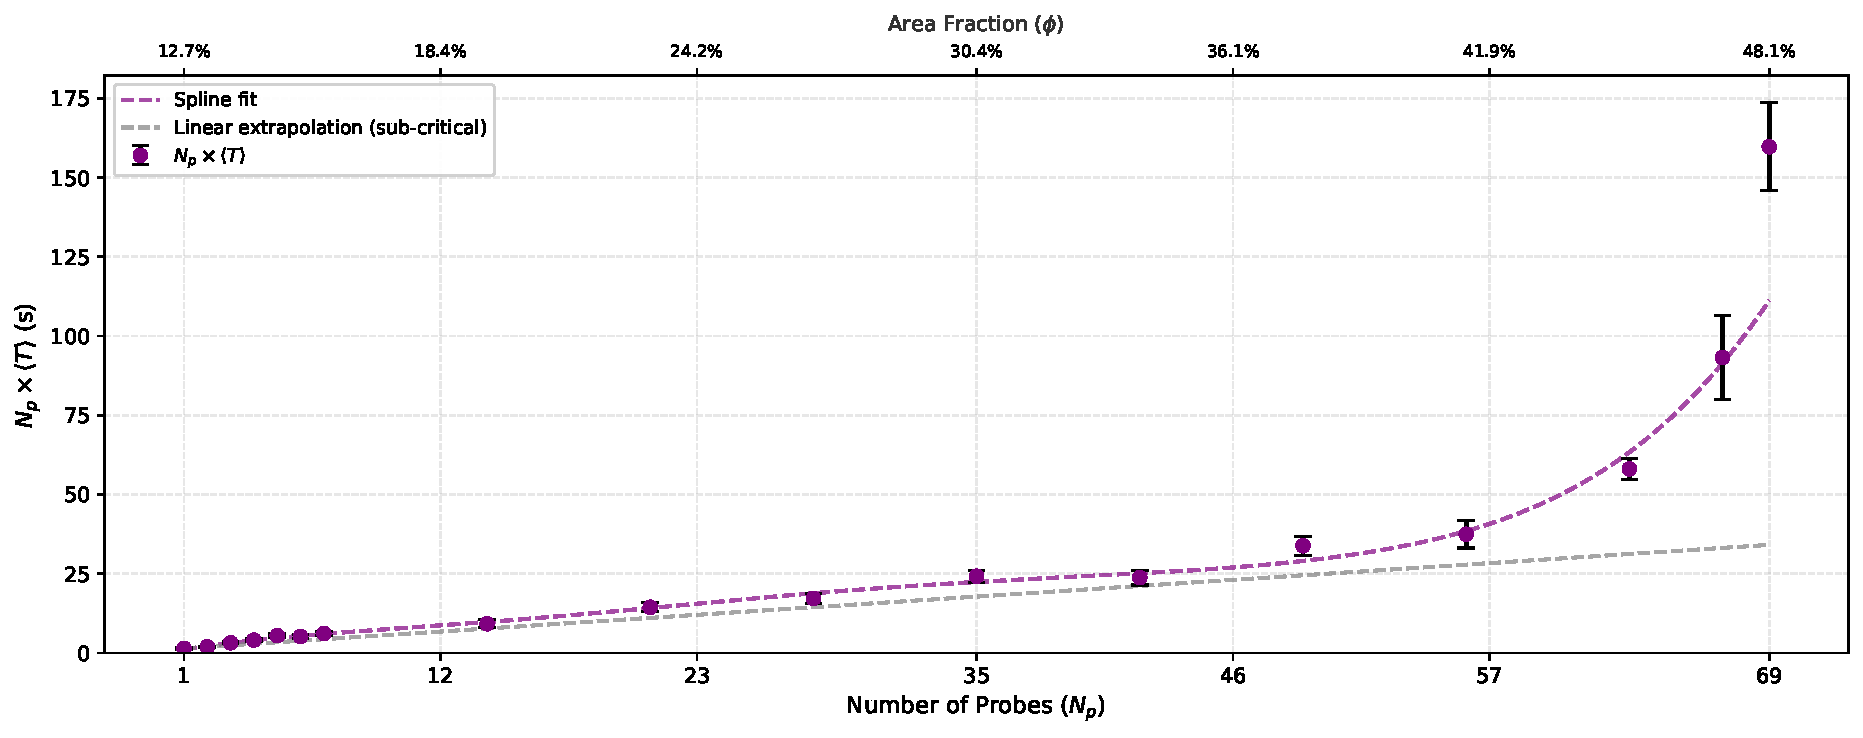
\includegraphics[width = 0.95\linewidth]{figures/ergodic_individual_N_70.pdf}
    \caption{Ergodic product $E = N_p\times \langle T\rangle$ versus $N_p$ and $\phi$ for the $N_\text{total} = 70$ system. The dashed line is a linear extrapolation of $E$ from the most dilute (sub-critical) points, representing the ideal, non-interacting-searcher expectation; the spline traces the actual measured values, and its upward departure from the extrapolation signals the onset of non-ergodic, crowding-influenced search.}
    \label{fig:ErgodicProduct70}
\end{figure}

\textbf{Figure~\ref{fig:ErgodicProduct70}} ($N_\text{total} = 70$) shows the first system where the departure is sharp and unambiguous. $E$ hugs its extrapolation almost exactly out to roughly $N_p = 46$, then bends away clearly, with error bars small enough relative to the separation that the last four or five points sit entirely above the extrapolation line rather than merely trending above it. By the final point ($N_p = 69$), the measured $E$ is roughly 1.5$\times$ its extrapolated value.

\begin{figure}[htbp]
    \centering
    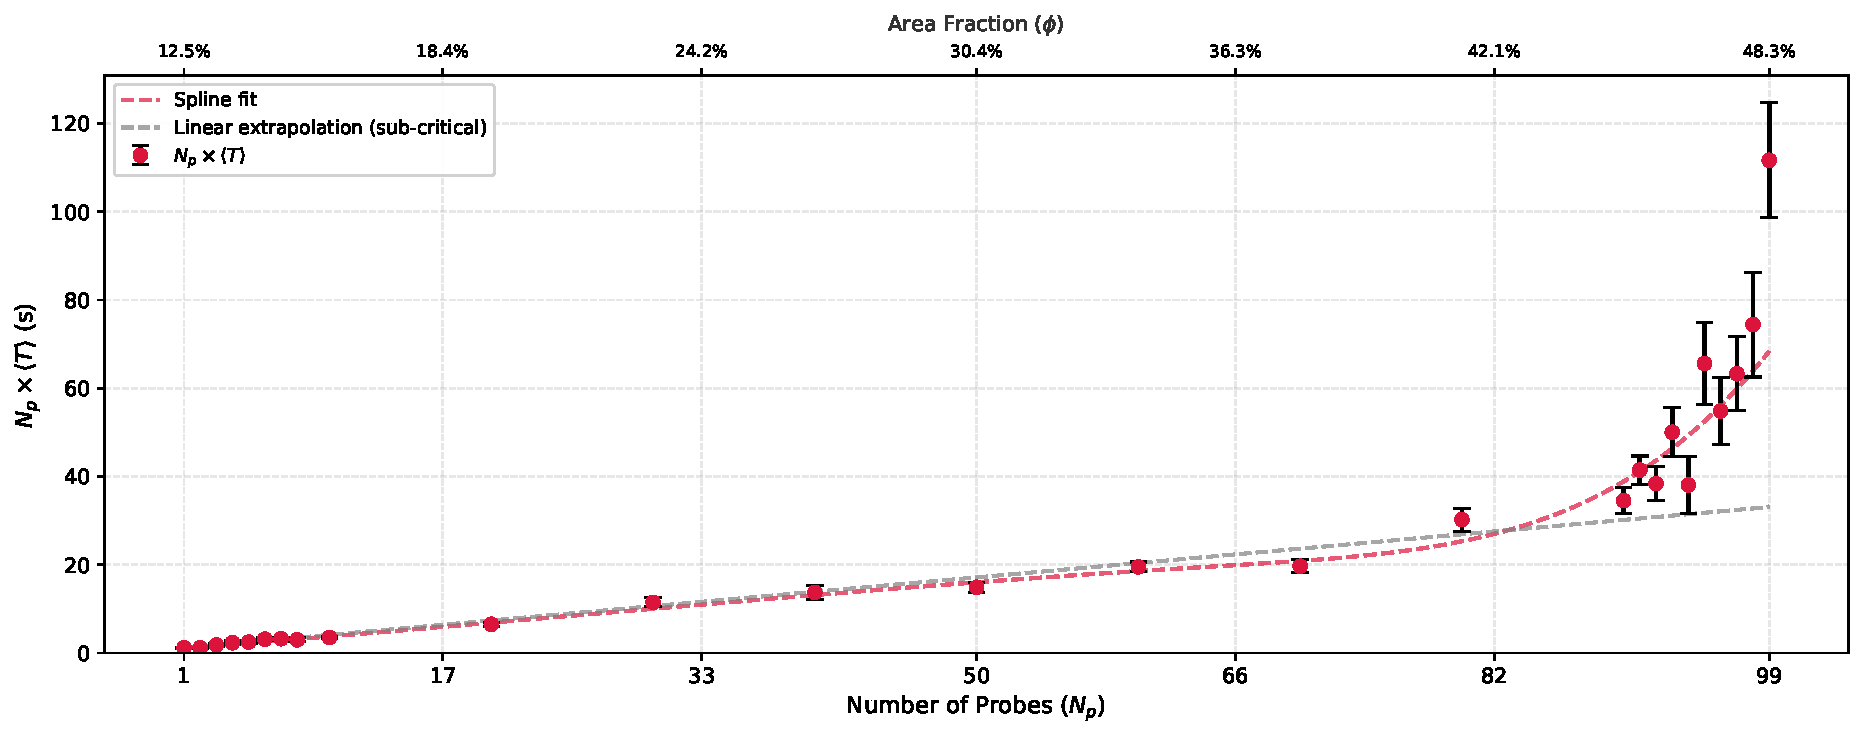
\includegraphics[width = 0.95\linewidth]{figures/ergodic_individual_N_100.pdf}
    \caption{Ergodic product $E = N_p\times \langle T\rangle$ versus $N_p$ and $\phi$ for the $N_\text{total} = 100$ system. The dashed line is a linear extrapolation of $E$ from the most dilute (sub-critical) points, representing the ideal, non-interacting-searcher expectation; the spline traces the actual measured values, and its upward departure from the extrapolation signals the onset of non-ergodic, crowding-influenced search.}
    \label{fig:ErgodicProduct100}
\end{figure}

\textbf{Figure~\ref{fig:ErgodicProduct100}} ($N_\text{total} = 100$) have twenty sampled points where this plot shows the departure most cleanly of any system. $E$ sits on its extrapolation, within tight error bars, through roughly $N_p = 66$, then visibly separates by  $N_p \approx 70$--82, and continues climbing steeply to end near 100--200\,s by $N_p = 99$, several multiples above the extrapolated value at that point. This departure is visible well before the corresponding upturn is unambiguous in $\langle T \rangle$ itself (Figure~\ref{fig:Caldera100}), a comparison developed in Section~\ref{sec:4.8}.

\begin{figure}[htbp]
    \centering
    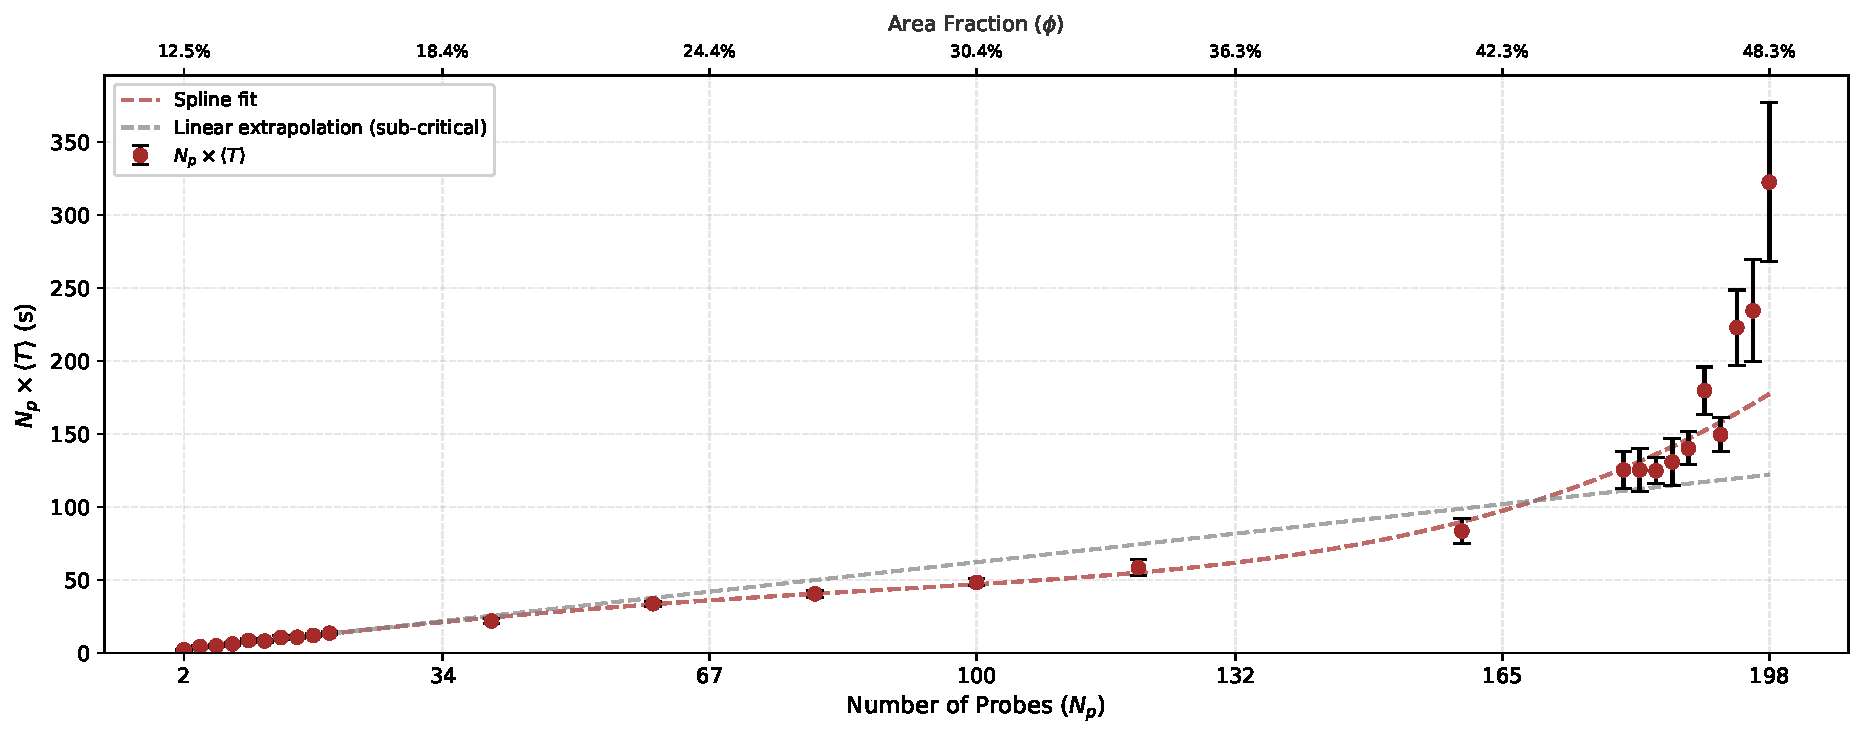
\includegraphics[width = 0.95\linewidth]{figures/ergodic_individual_N_200.pdf}
    \caption{Ergodic product $E = N_p\times \langle T\rangle$ versus $N_p$ and $\phi$ for the $N_\text{total} = 200$ system. The dashed line is a linear extrapolation of $E$ from the most dilute (sub-critical) points, representing the ideal, non-interacting-searcher expectation; the spline traces the actual measured values, and its upward departure from the extrapolation signals the onset of non-ergodic, crowding-influenced search.}
    \label{fig:ErgodicProduct200}
\end{figure}

\textbf{Figure~\ref{fig:ErgodicProduct200}} ($N_\text{total} = 200$) shows the dramatic absolute departure as the largest system. $E$ tracks its extrapolation closely out to roughly $N_p = 132$, then rises sharply, ending above 300\,s by the final sampled points near $N_p \approx 190$--198 which is more than double the extrapolated value at that $N_p$. The error bars widen substantially over the last several points but remain small relative to the size of the departure itself, leaving no ambiguity that $E$ has broken from the ideal, non-interacting-searcher scaling well before the sweep ends.

\begin{figure}[htbp]
    \centering
    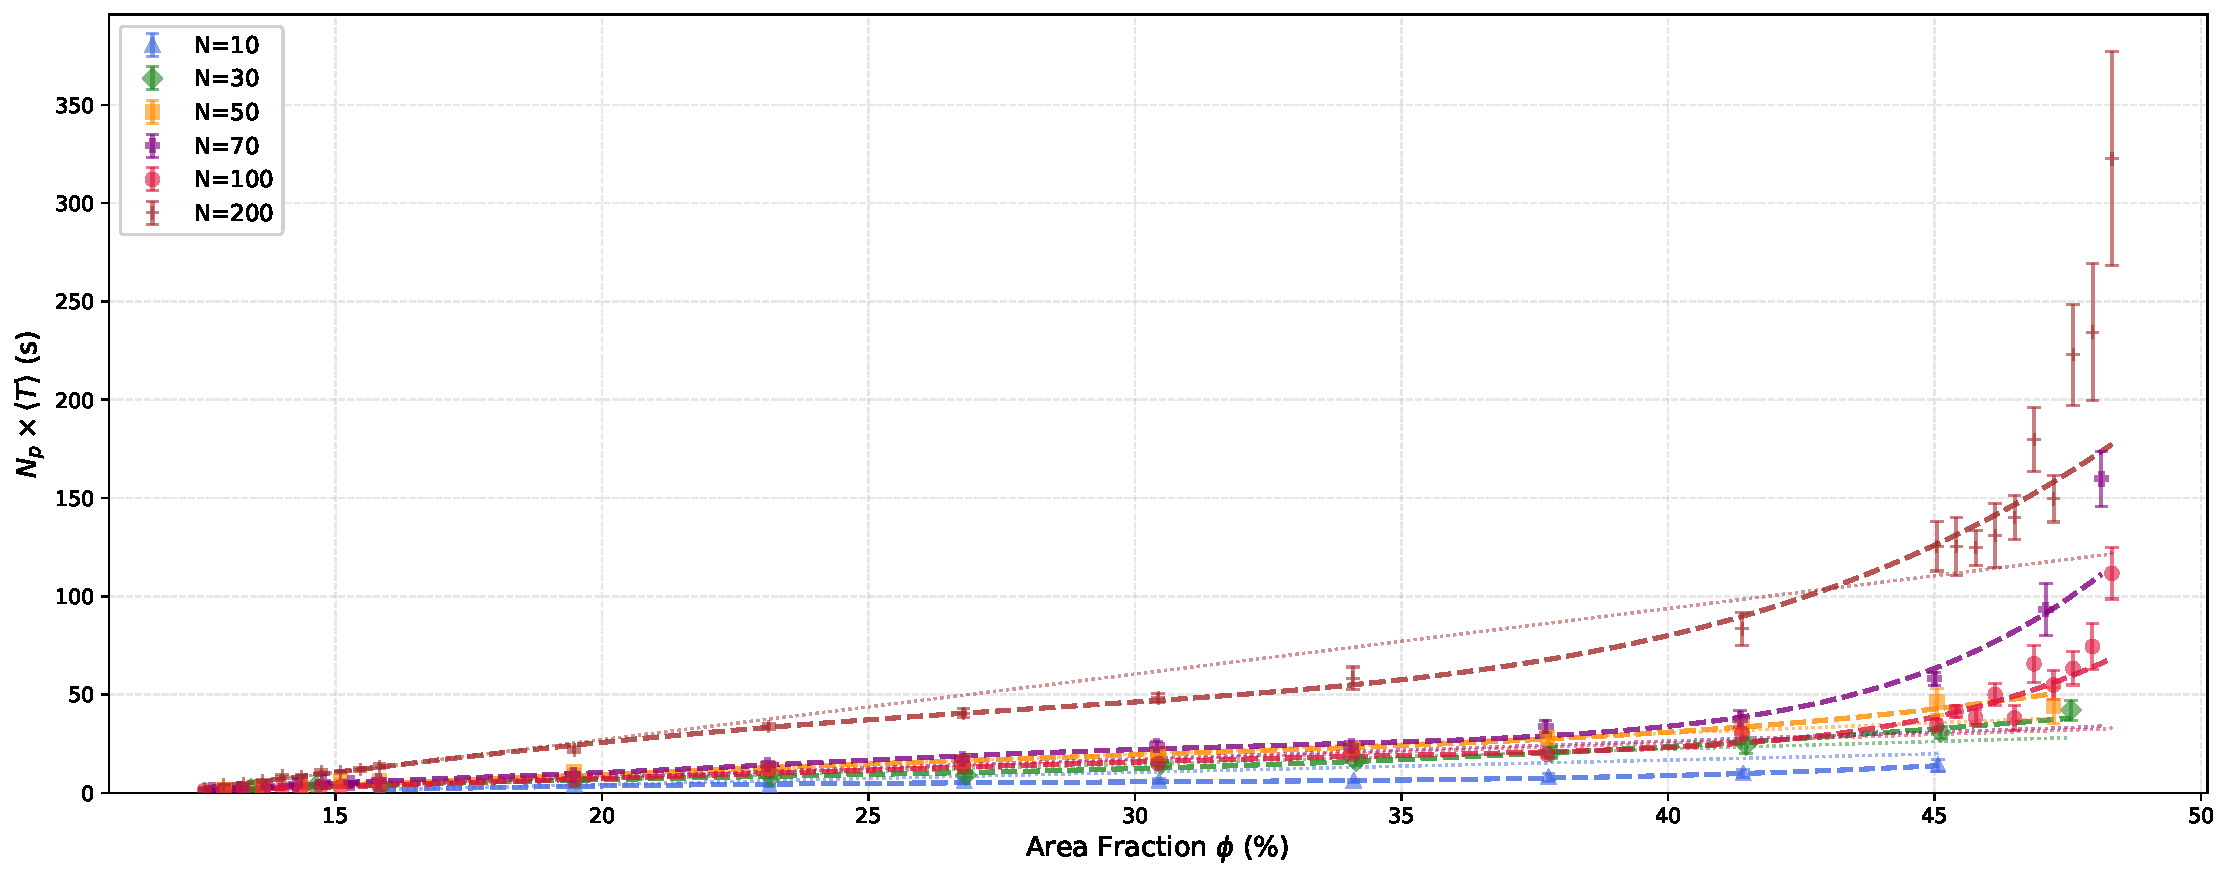
\includegraphics[width = 0.95\linewidth]{figures/FigB_ergodic_overlay.pdf}
    \caption{Overlay of the ergodic product $E = N_p \times \langle T \rangle$ versus area fraction $\phi$ for all six system sizes, illustrating that the departure from ideal, ergodic $1/N_p$ scaling occurs at a similar $\phi$ across systems despite the very different absolute magnitudes of $E$.}
    \label{fig:OverlayErgodicProduct}
\end{figure}

\textbf{Figure~\ref{fig:OverlayErgodicProduct}} shows the six ergodic-product curves placed on a common $\phi$ axis
spanning more than an order of magnitude in absolute scale, from roughly 20\,s at $N_\text{total} = 10$ to over 300\,s at $N_\text{total} =200$, yet all six begin bending away from linear growth in roughly the same window of area fraction, visually clustered between about $\phi\approx 30\%$ and $45\%$. The larger systems ($N_\text{total} = 70, 100, 200$) show the clearest, most steeply rising departures in this view, consistent with their sharper individual plots above, while the $N_\text{total} = 10$ and 30 curves remain closer to their respective extrapolations across most of the shared axis, only diverging visibly at the highest sampled $\phi$.

The clarity of the sub-critical-extrapolation departure differs markedly by system size. In the $N_\text{total} =10$ and 30 systems, the departure is gradual and its error bars are wide enough relative to the signal that an unambiguous departure point is difficult to identify. In the $N_\text{total} =70$, 100, and 200 systems, by contrast, the departure is sharp and resolvable well within the error bars, and, importantly, it becomes visible at a lower $N_p$ than the corresponding upward inflection in the raw $\langle T \rangle$ curve of Section~\ref{sec:4.2}. For the $N_\text{total} =100$ system, $E$ departs visibly from its extrapolation by rought $N_p \approx 70$--80, while the equivalent upturn does not become visually unambiguous in $\langle T\rangle$ itself (Figure~\ref{fig:Caldera100}) until closer to $N_p \approx 90$ which gives ergodic product a lead of some twenty to thirty probes. A comparable lead is visible for $N_\text{total}=200$ (departure near $N_p \approx 150$--165 in Figure~\ref{fig:ErgodicProduct200}, versus a visible $\langle T \rangle$ upturn closer to $N_p \approx 180$ in Figure~\ref{fig:Caldera200}).

\section{Detection Time Distributions: The Violin Plots}
\label{sec:4.5}

\begin{figure}[htbp]
    \centering
    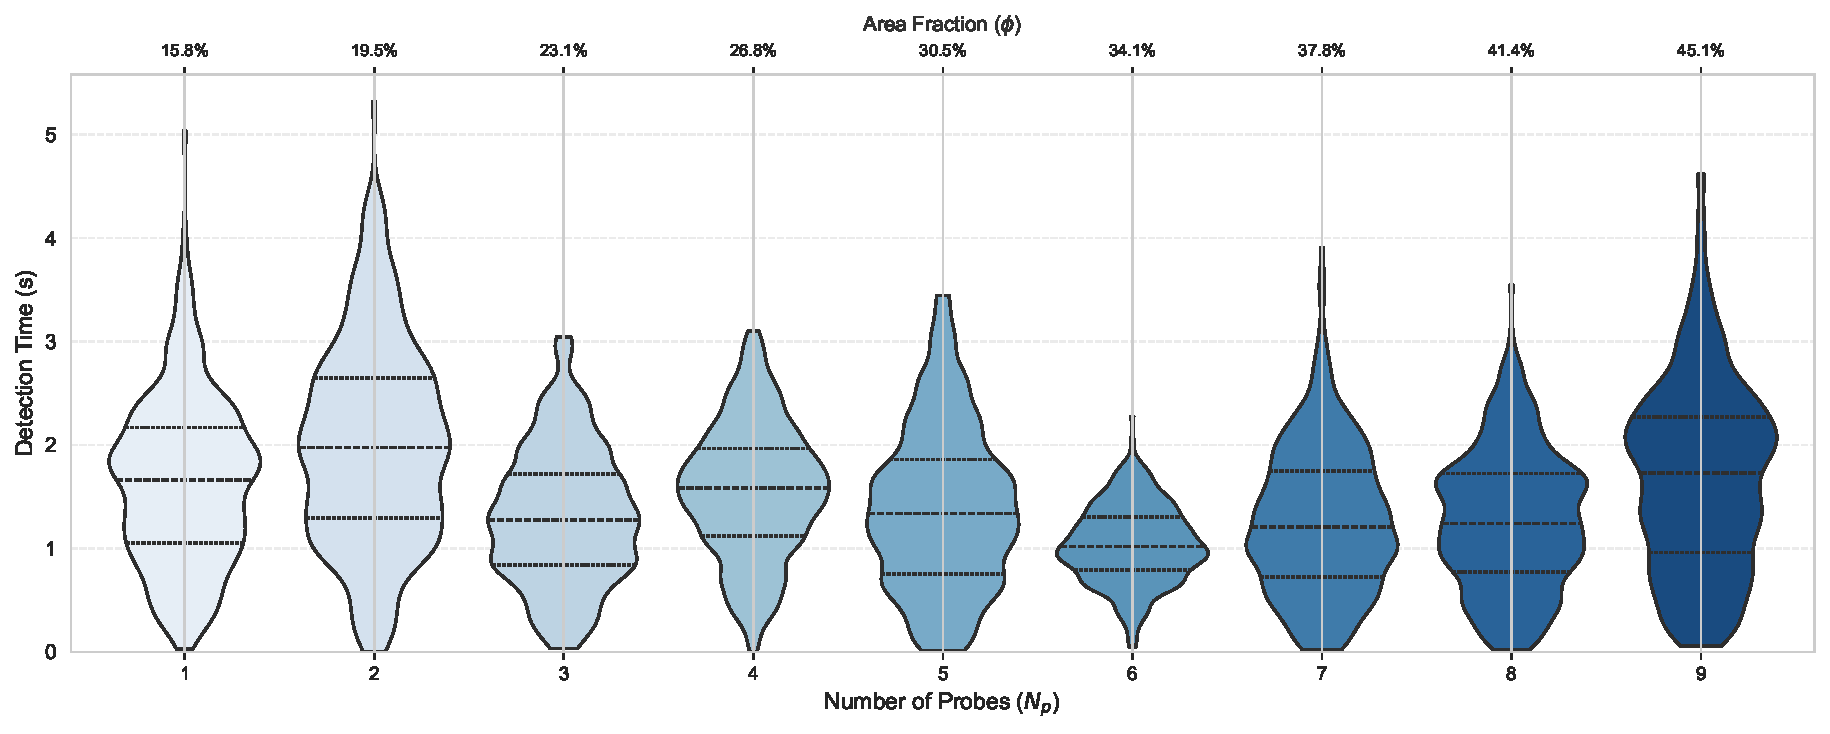
\includegraphics[width = 0.95\linewidth]{figures/violin_individual_N_10.pdf}
    \caption{Violin plots of the first-passage detection-time distribution as a function of probe number $N_p$ (bottom axis) and area fraction $\phi$ (top axis) for the $N_\text{total} = 10$ system, with each violin generated from a Gaussian approximation matched to that condition's ensemble mean and standard deviation (Section~\ref{sec:3.11}).}
    \label{fig:Violin10}
\end{figure}

\textbf{Figure~\ref{fig:Violin10}} ($N_\text{total} = 10$) shows nine violins who are all comparatively wide relative to their medians, consistent with this system's small ensemble and coarse $N_p$ sampling noted in Section~\ref{sec:4.1}. The narrowest violin occurs near $N_p = 6$, matching the fitted optimum in Table~\ref{tab:caldera-optima}, but the difference in width between this violin and its neighbors is modest where the widest and most visibly asymmetric violin appears at the crowded end, $N_p =9$, where the upper tail extends well past 4\,s.


\begin{figure}[htbp]
    \centering
    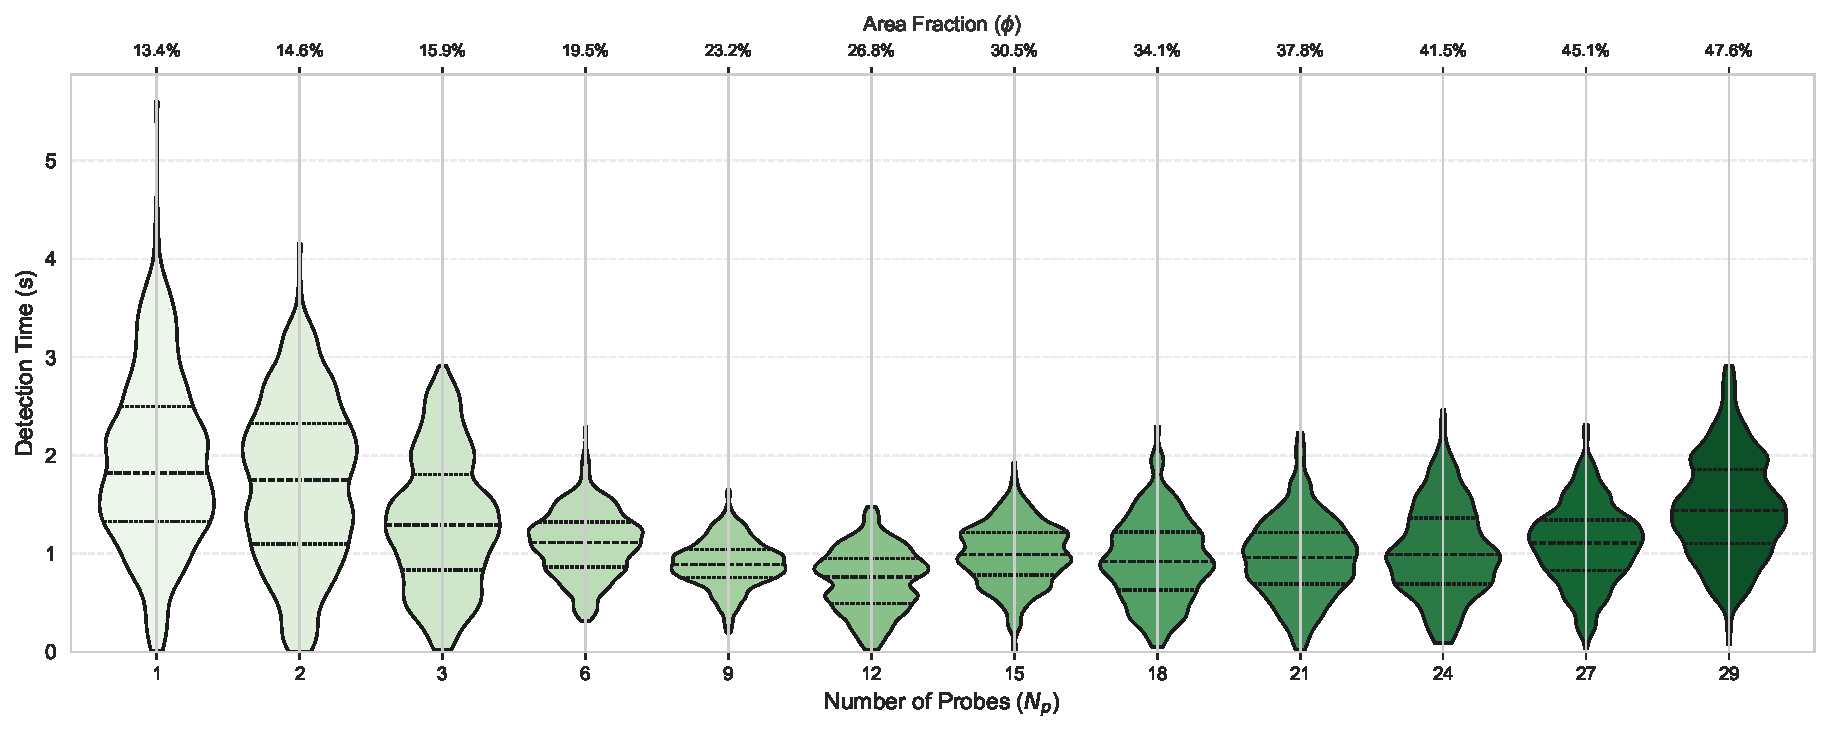
\includegraphics[width = 0.95\linewidth]{figures/violin_individual_N_30.pdf}
    \caption{Violin plots of the first-passage detection-time distribution as a function of probe number $N_p$ (bottom axis) and area fraction $\phi$ (top axis) for the $N_\text{total} = 30$ system, with each violin generated from a Gaussian approximation matched to that condition's ensemble mean and standard deviation (Section~\ref{sec:3.11}).}
    \label{fig:Violin30}
\end{figure}

\textbf{Figure~\ref{fig:Violin30}} ($N_\text{total} = 30$) shows a progression from wide to narrow to wide again that is clearer here than at $N_\text{total} =10$. The $N_p =1$--2 violins are tall and diffuse, the distribution from roughly $N_p =9$ to $18$ are visibly the most compact of the set, and the violins broaden again gradually toward $N_p = 29$, though the final violin remains narrower and less skewed than the crowded-end violins of the larger systems described below.

\begin{figure}[htbp]
    \centering
    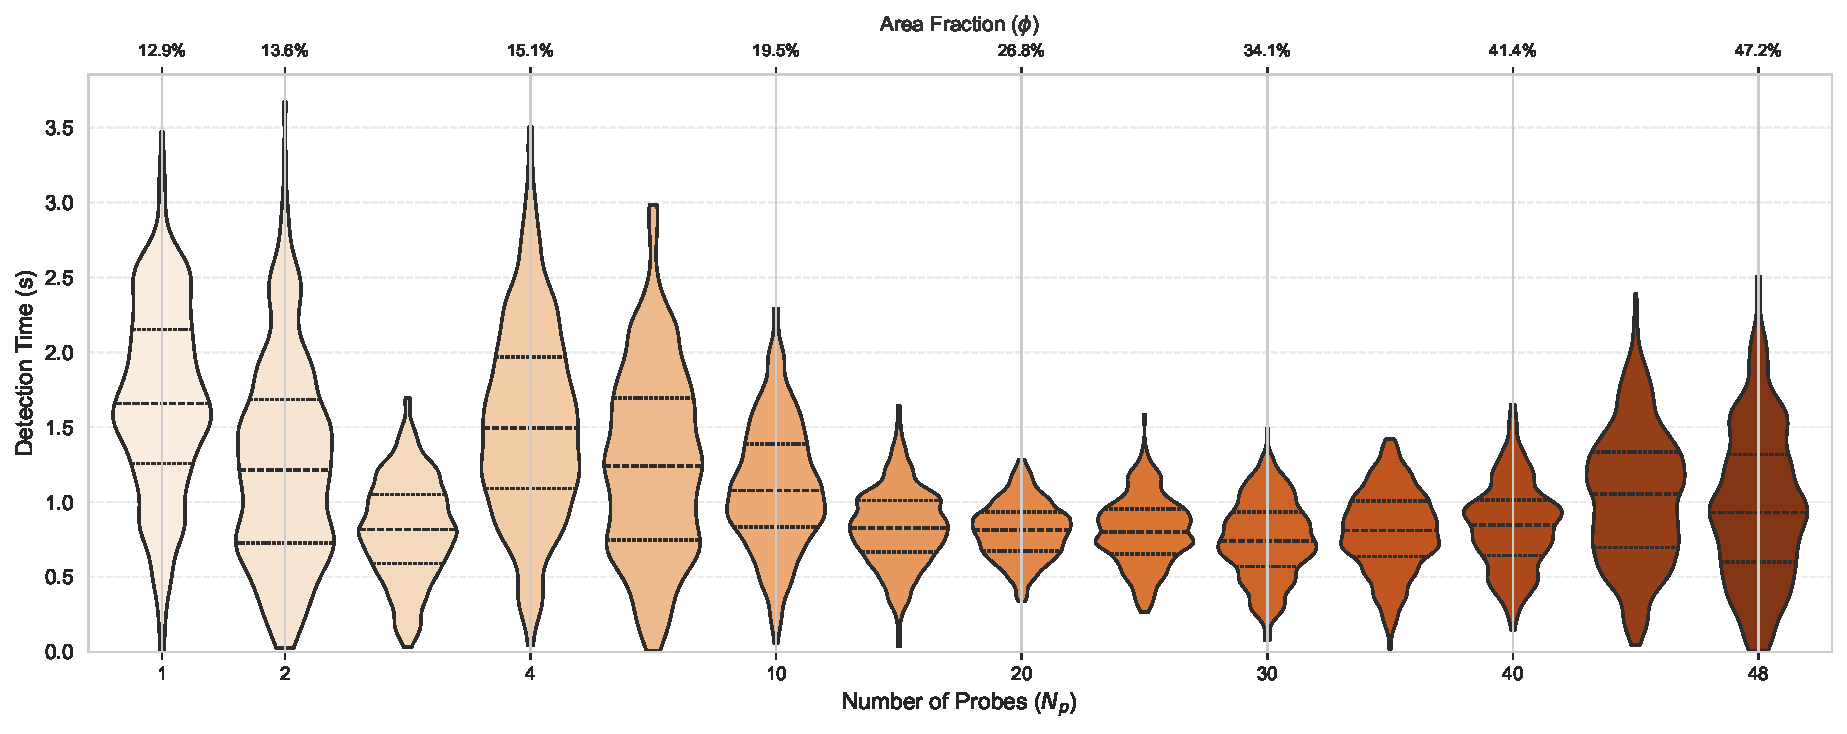
\includegraphics[width = 0.95\linewidth]{figures/violin_individual_N_50.pdf}
    \caption{Violin plots of the first-passage detection-time distribution as a function of probe number $N_p$ (bottom axis) and area fraction $\phi$ (top axis) for the $N_\text{total} = 50$ system, with each violin generated from a Gaussian approximation matched to that condition's ensemble mean and standard deviation (Section~\ref{sec:3.11}).}
    \label{fig:Violin50}
\end{figure}

\textbf{Figure~\ref{fig:Violin50}} ($N_\text{total} = 50$) shows that the violins at $N_p = 1$ and, especially, $N_p =4$ are the talles and most visibly right-skewed of the dilute-end conditions, echoing the early non-monotonicity seen in $\langle T \rangle$ for this system (Figure~\ref{fig:Caldera50}). The distributions tighten substantially from roughly $N_p =10$ through $30$, forming the flattest, most symmetric stretch the violins in the plot, before widening again at $N_p = 40$ and 48, where the upper tails begin to extend visibly beyond 2\,s.

\begin{figure}[htbp]
    \centering
    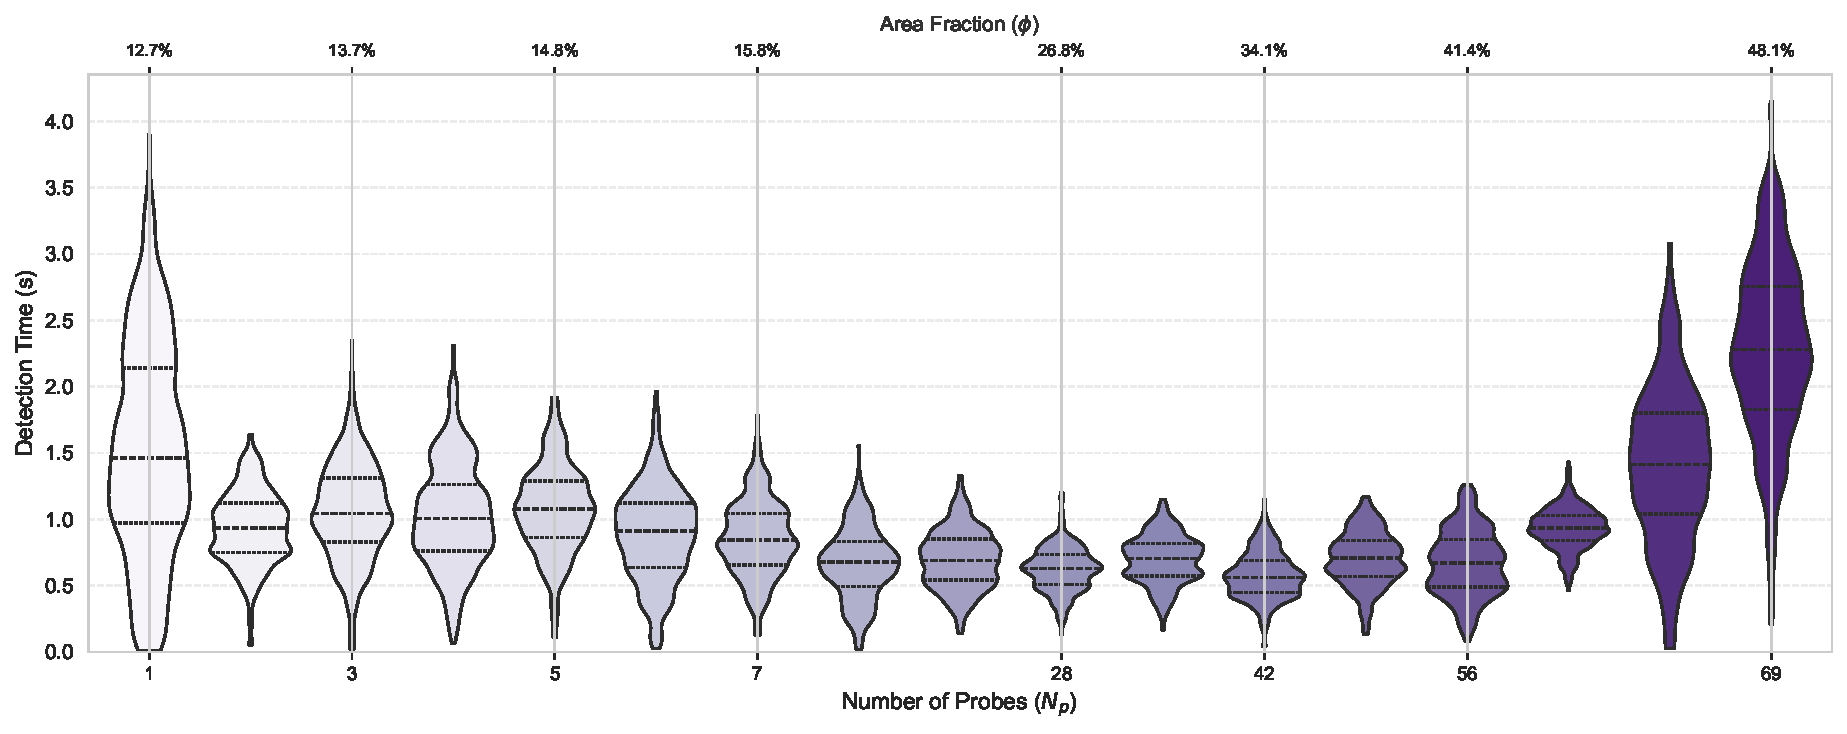
\includegraphics[width = 0.95\linewidth]{figures/violin_individual_N_70.pdf}
    \caption{Violin plots of the first-passage detection-time distribution as a function of probe number $N_p$ (bottom axis) and area fraction $\phi$ (top axis) for the $N_\text{total} = 70$ system, with each violin generated from a Gaussian approximation matched to that condition's ensemble mean and standard deviation (Section~\ref{sec:3.11}).}
    \label{fig:Violin70}
\end{figure}

\textbf{Figure~\ref{fig:Violin70}} ($N_\text{total} = 70$) shows violins with the contrast between the flat middle of the sweep and its crowded edge is the sharpest yet. The violin from roughly $N_p = 7$ through $58$ are visibly compact and close to symmetric, while the final two violins, at $N_p = 69$ and the point just before it, are both taller and more clearly right-skewed than any distribution earlier in the sweep, with upper tails reaching past 3\,s while the bulk of the density remains below 1.5\,s.

\begin{figure}[htbp]
    \centering
    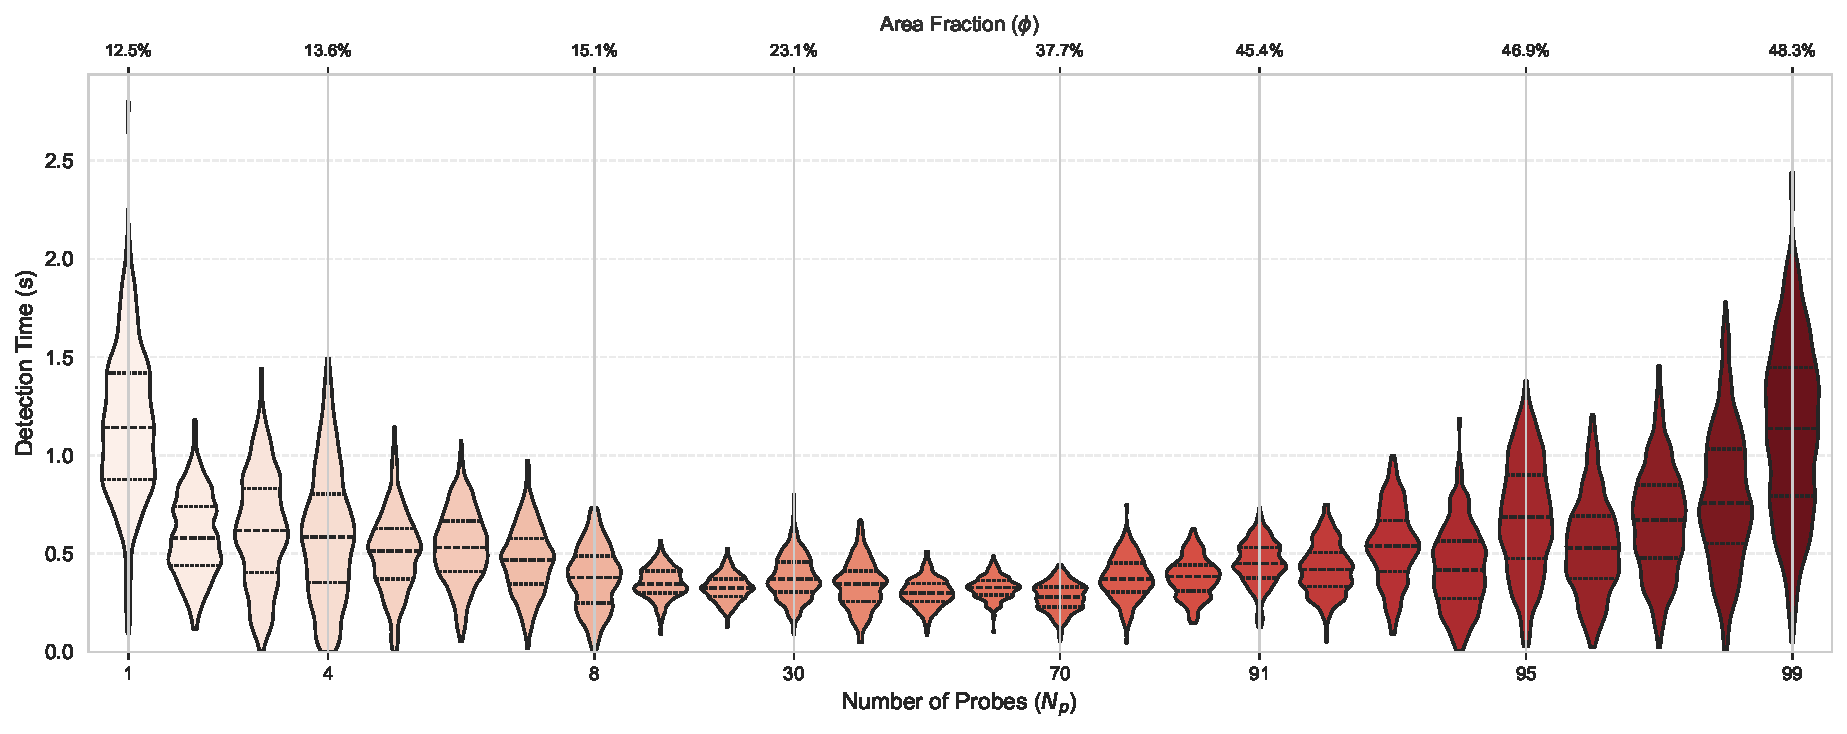
\includegraphics[width = 0.95\linewidth]{figures/violin_individual_N_100.pdf}
    \caption{Violin plots of the first-passage detection-time distribution as a function of probe number $N_p$ (bottom axis) and area fraction $\phi$ (top axis) for the $N_\text{total} = 100$ system, with each violin generated from a Gaussian approximation matched to that condition's ensemble mean and standard deviation (Section~\ref{sec:3.11}).}
    \label{fig:Violin100}
\end{figure}

\textbf{Figure~\ref{fig:Violin100}} ($N_\text{total} = 100$) shows twenty violins plotted and the clearest gradual narrowing and re-widening of the six systems. The violin width decreases steadily from $N_p =1$ to a visibly flat, thin band spanning roughly $N_p 3=0$ to $70$, then re-expands progressively toward $N_p = 99$. The last three or four violins are also the most visibly right-skewed of the set up to this point in the sweep, with medians that shift upward alongside the widening tails which is a shape echoed even more strongly in the $N_\text{total} =200$ system below.

\begin{figure}[htbp]
    \centering
    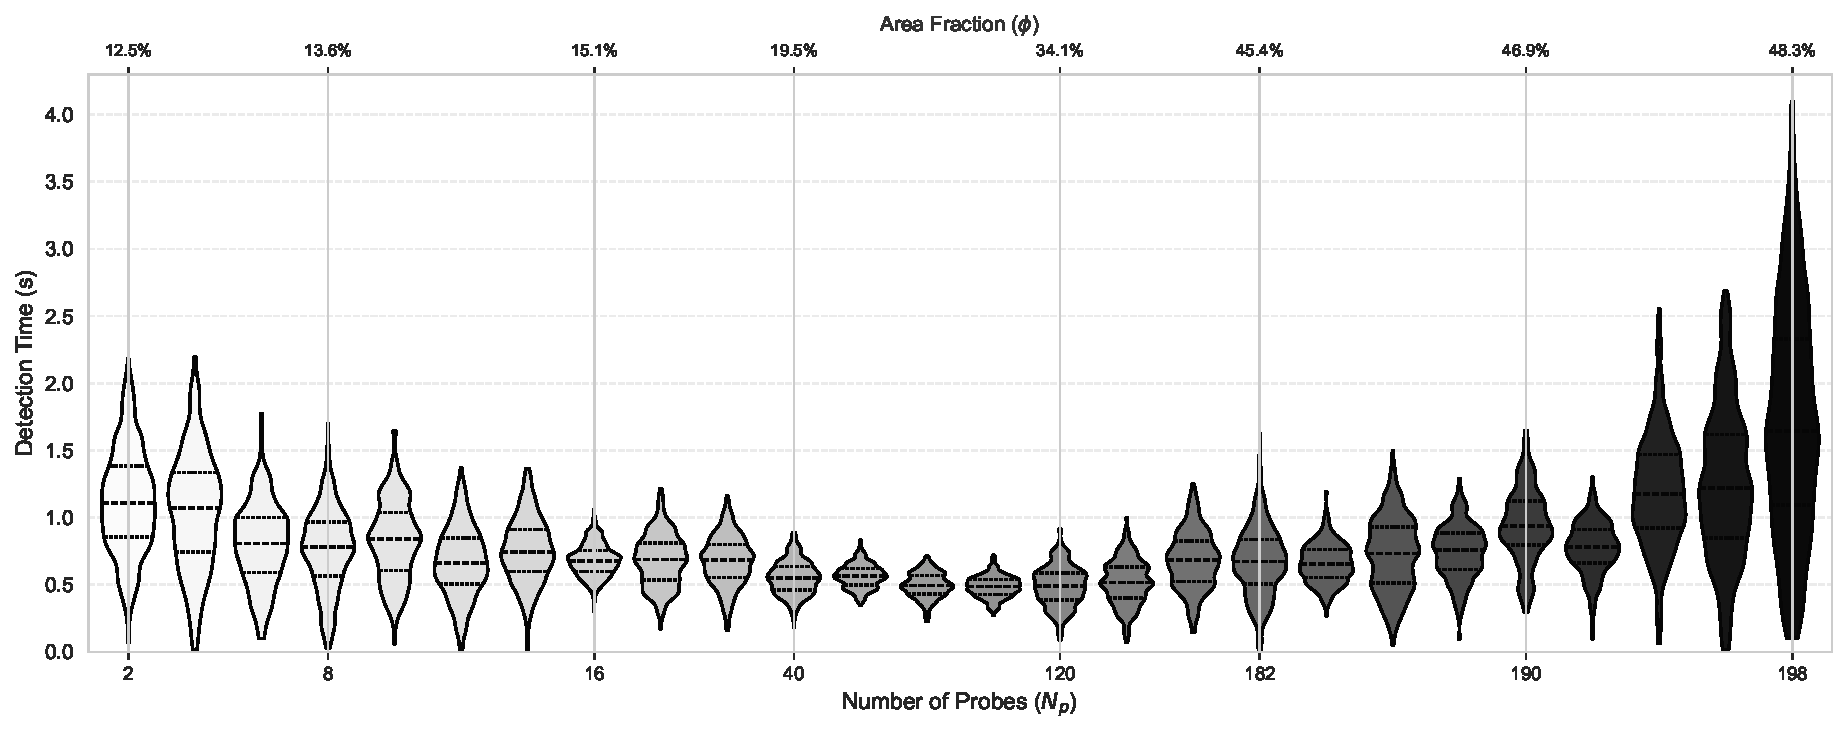
\includegraphics[width = 0.95\linewidth]{figures/violin_individual_N_200.pdf}
    \caption{Violin plots of the first-passage detection-time distribution as a function of probe number $N_p$ (bottom axis) and area fraction $\phi$ (top axis) for the $N_\text{total} = 200$ system, with each violin generated from a Gaussian approximation matched to that condition's ensemble mean and standard deviation (Section~\ref{sec:3.11}). Showing the most pronounced broadening and right-skewing of any system size at the most crowded conditions sampled.}
    \label{fig:Violin200}
\end{figure}

\textbf{Figure~\ref{fig:Violin200}} ($N_\text{total} = 200$) shows the most dramatic distributional change of the entire sweep. The violins across the broad middle of the range (roughly $N_p =40$ to $165$) are thin, symmetric, and nearly indistinguishable from one another in shape, but the final several violins, from around $N_p = 182$ onward, grow markedly taller and visibly right-skewed, with the $N_p = 198$ violin extending past 4\,s while its median remains well below that value showing the clearest visual signature in this thesis of a small number of runs taking substantially longer to detect than the typical run at the same condition.

\begin{figure}[htbp]
    \centering
    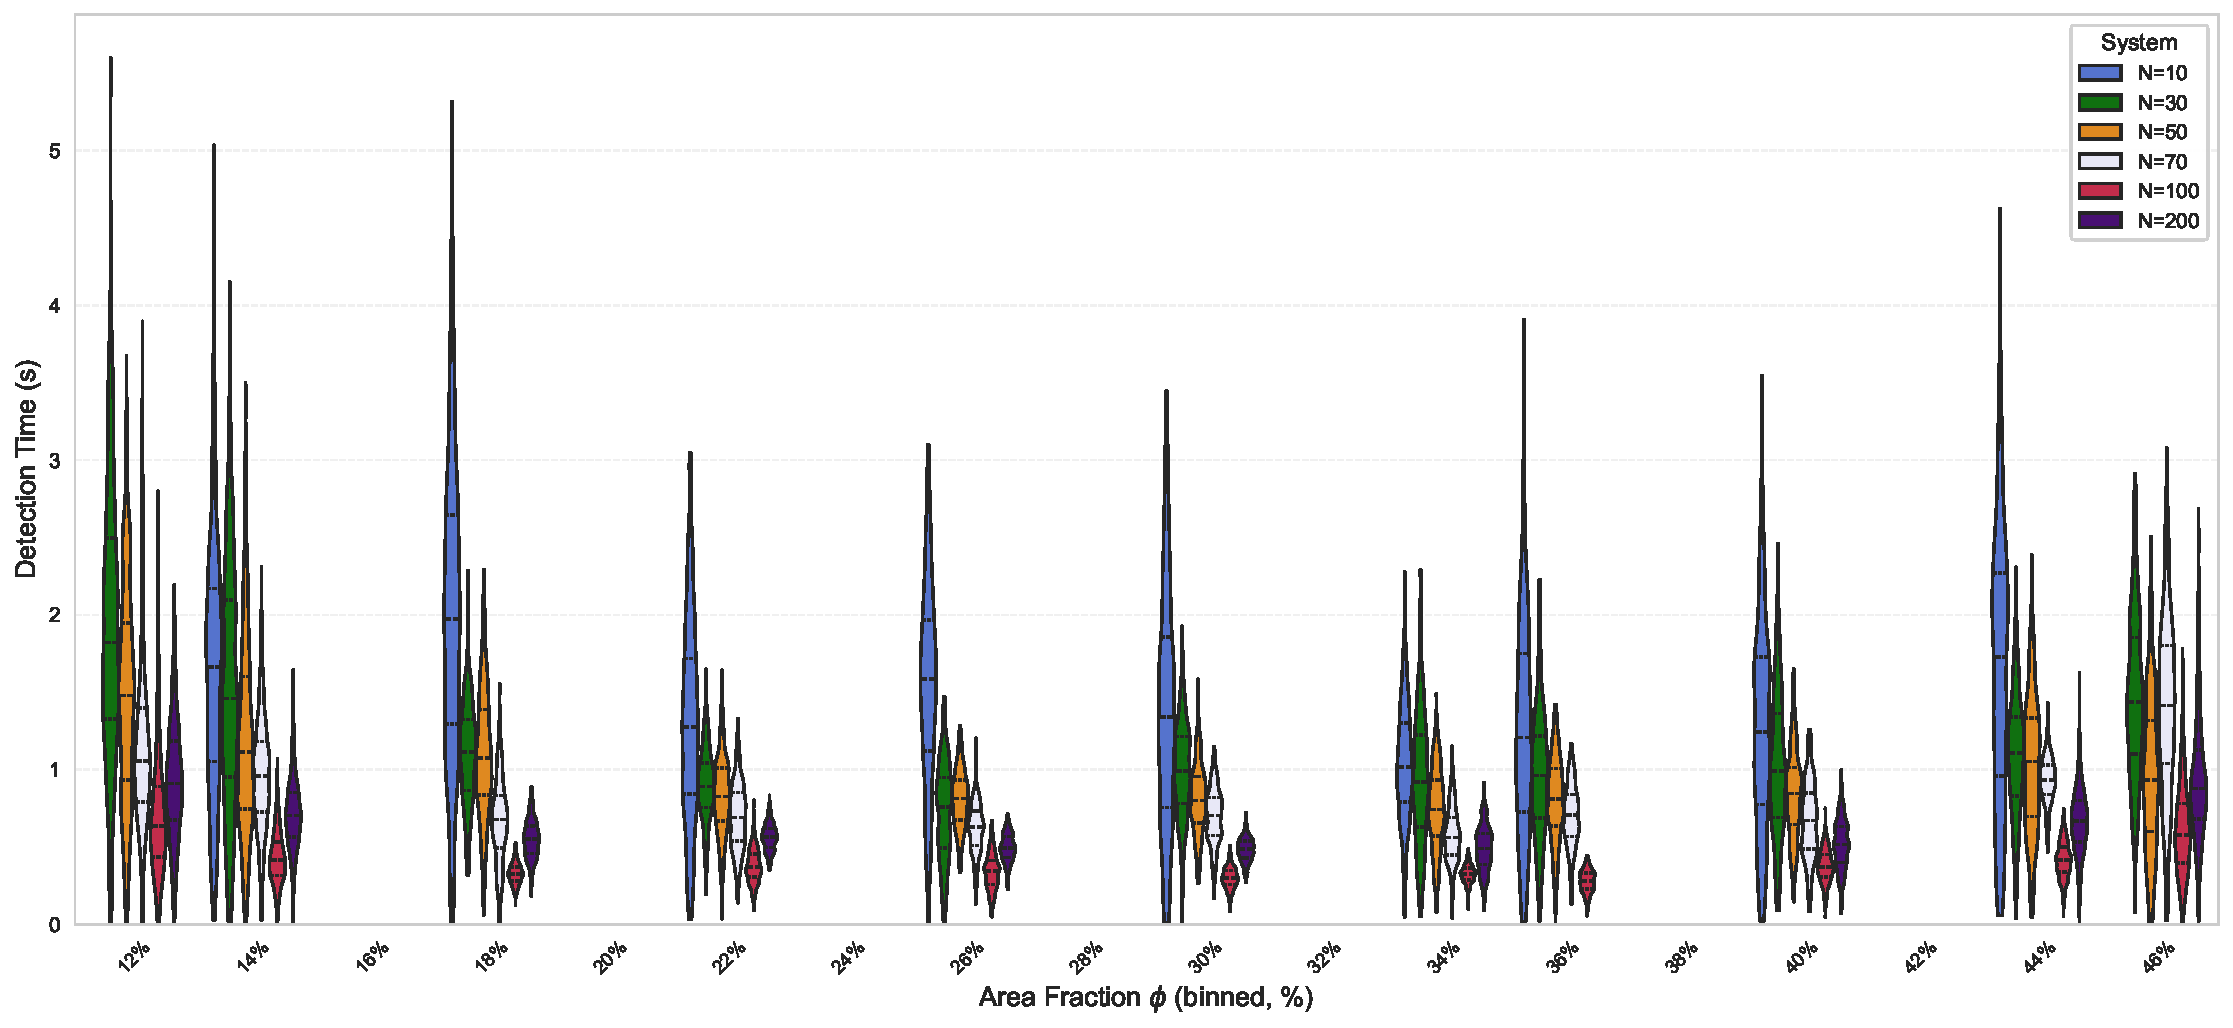
\includegraphics[width = 0.95\linewidth]{figures/FigD_violin_overlay.pdf}
    \caption{Composite violin plot comparing the detection-time distribution across all six system sizes, binned by area fractions $\phi$, with each system color-coded. This view shows how both the central tendency and the shape of the distribution evolve with crowding consistently across system scales.}
    \label{fig:OverlayViolin}
\end{figure}

\textbf{Figure~\ref{fig:OverlayViolin}} bins all six systems onto a common $\phi$ axis showing that, despite their very different absolute $N_p$ ranges, the six color-coded families of violins narrow toward their individually tightest shapes in roughly the same middle bins of the shared axis (broadly $\phi \approx 20$--35\%) and widen again together in the bins beyond about $\phi \approx 40\%$. The $N_\text{total} = 10$ family (narrowest range of bins populated, owing to its coarse sampling) and the $N_\text{total} = 200$ family (populating the most bins, and showing the tallest, most skewed violins at the crowded end) sit at opposite extremes of this composite view, with the four intermediate system sizes arranged between them in a consistent, overlapping progression.

Taken together, the violin plots (Figures~\ref{fig:Violin10}--\ref{fig:OverlayViolin}) show a consistent evolution in distribution shape across the prove-density sweep, in every system. Broad and occasionally asymmetric distribution at the dilute end ($N_p = 1$--2), narrowing to their tightest and most symmetric near the caldera floor, and broadening  again, with visible right-skew, toward the crowded end of the sweep. The severity of this crowded-end broadening differs by system size. The $N_\text{total} = 200$ system shows the most pronounced broadening and right-skewing of any system at its most crowded sampled conditions, while the $N_\text{total} =10$ system shows comparatively modest change in shape between its floor and crowded-end violins. The composite plot binned by area fraction shows that this evolution in shape occurs at a similar $\phi$ across system sizes, reinforcing $\phi$, rather than raw $N_p$ or $N_\text{total}$, as the more natural variable for comparing search behavior across scales.

\section{Typology for the Caldera profiles}
\label{sec:4.6}

Four types of "caldera" inspired by volcanology.

\textbf{Type I - Incipient (Latent) Caldera.} A minimum exists in the fit, but the apparent rise on the crowded side is comparable to or smaller than the run-to-run standard error, so the crowding side cannot be distinguished from statistical noise given ten seeds and the coarse, low-Np integer sampling available at small $N_\text{total}$. What's included here is $N_\text{total} = 10$.

\textbf{Type II - Shield Caldera.} The minimum is statistically resolvable and a genuine, monotonic rise appears at high $N_p$, but the rise is modest. a broad, gently sloping floor rather than a sharp wall, with the crowded-side $\langle T \rangle$ reaching only roughly 1.1-1.8$\times$ the floor value. What's included here are $N_\text{total} = 30$ and 50.

\textbf{Type III - Steep-Walled (Stratovolcano) Caldera.} A long, flat, low-variance diffusion limited plateau in a sharp, unambiguous upturn near the top of the sampled Np range, with $\langle T \rangle$ rising to roughly 2-5$\times$ the floor value and the standard deviation widening in step. The ergodic product for these systems also breaks from its sub-critical extrapolation well before the rise is visible in $\langle T \rangle$ alone. Examples of this type of caldera includes $N_\text{total} = 70$, 100, 200.

\textbf{Type IV - Bifurcated (Double-floor) Caldera}. A small number of systems display a caldera floor that does not settle into a single, uninterrupted minimum. Instead, the $\langle T \rangle$ versus $N_p$ profile dips to a first low point, rises gently, and dips again to a second low point before finally climbing into the crowding-limited regime on the far side. Visually, this resembles a caldera with two adjacent low points along its floor rather than one continuous basin. The clearest of this pattern appears in the $N = 100$ system, where a shallow first floor near $N_p\approx 15$--20 is followed by a modest rise and then a deeper second floor near $N_p \approx 50$--70. A weaker, less pronounced version of the same shape is also visible in the $N=70$ profile. We introduce Type IV here as a qualitative addition to the caldera typology, identified descriptively by its floor shape in the same manner as Types I, II, and III.

This typology is not confined to the caldera fit alone, it is corroborated by the other two diagnostics. The Type I system ($N_\text{total} = 10$) show sthe least resolvable departure in the ergodic product (Section~\ref{sec:4.4}) and the least dramatic change in violin shape (Section~\ref{sec:4.5}) between its floor and crowded conditions. The Type II systems ($N_\text{total} = 30$, 50) show a modest but genuine departure in both. The Type III systems ($N_\text{total} = 70$, 100, 200) show sharp, well-resolved signatures across all three diagnostics simultaneously --- the caldera fit, the ergodic product, and the violin plot broadening all sharpen together as system size grows.

\section{The Agreement of the Three Diagnostics}
\label{sec:4.7}

Three methodologically independent diagnostics, being the parametric caldera fit's minimum (Section~\ref{sec:4.2}), the ergodic product's departure from ideal linear scaling (Section~\ref{sec:4.4}), and the qualitative broadening of the detection-time distribution (Section~\ref{sec:4.5}), converges on locating the crowding transition within a similar area-fraction band, roughly $\phi \approx 28$--35\%, across all six system sizes. This convergence matters because the three diagnostics make different assumptions. The caldera fit assumes a specific two-term functional form (Equation~\ref{eq:3.6}), the ergodic product assumes only that ideal search behaves as a flat line in $N_p$, and the violin-plot broadening assumes nothing beyond the shape of the sampled distribution itself. That three routes with little in common beyond the underlying data arrive at the same transition window makes it unlikely that $\phi^* \approx 30\%$ is an artifact of any single analytical choice, such as the exponents or amplitude bounds used in the nonlinear least-squares fit. The agreement is tightest for the Type III systems ($N_\text{total} = 70,100,200$), where all three diagnostics are individually well-resolved and mutually consistent. The agreement is loosest for the Type I and Type II systems ($N_\text{total}= 10, 30, 50$), where each diagnostic is individually less statistically confident, a limitation attributable to the small number of discrete $N_p$ values available at low $N_\text{total}$ (Section~\ref{sec:3.1}) rather than to any disagreement in the underlying physics.

\section{Sensitivity Hypothesis Confirmation}
\label{sec:4.8}
Section~\ref{sec:1.3} posed the ergodic product as a candidate for detecting the onset of crowding earlier than $\langle T \rangle$ alone. The results in Section~\ref{sec:4.4} confirm this, at least for the Type III systems where $E$ departs from its ideal linear extrapolation some twenty to thirty probes before the corresponding rise is visually unambiguous in the raw $\langle T \rangle$ curve. A plausible mechanistic reason is that $E = N_p \times \langle T \rangle$ converts a small multiplicative deviation from ideal $1/N_p$ scaling directly into a deviation from a flat baseline, whereas the same deviation, expressed in $\langle T \rangle$ itself, is masked by the still-declining $1/N_p$ trend until the deviation grows large enough to visibly overcome that decline. In effect, $E$ re-expresses a subtle relative slowdown as an absolute, additive departure from a constant, which is easier to distinguish from measurement noise than the same slowdown buried in an already-falling curve. This sensitivity advantage is clearest for the systems with the most $N_p$ sampling points and the tightest error bars ($N_\text{total} = 70,100,200$). As for $N_\text{total} = 10$ and 30, the hypothesis is not denied, but the advantage cannot be established with confidence given the available sampling density which is an important caveat for any point-of-care application operating at low absolute particle counts, where the extra sensitivity this thesis reports may not be practically realizable.

\section{A complication for Ideal Search Theory}
\label{sec:4.9}
The ideal $1/N_p$ scaling law (Section~\ref{sec:2.3}) is a dilute-limit statement, and classical intuition about when that limit breaks down often defaults to geometric packing constraints which is also the assumption that searchers only meaningfully interfere with one another as the system approaches close packing. The results here complicate that intuition considerably. Across all six systems, the crowding-limited regime sets in within a band corroborated by all three diagnostic of Section~\ref{sec:4.7}, $\phi \approx28$--35\%, and most precisely located within that band by the parametric caldera fit at $\phi^* \approx 29$--31\% (Table~\label{ref:4.1}), roughly one-third of the hexagonal close-packing ceiling ($\phi_\text{HCP} \approx 90.7\%$, Section~\ref{sec:1.2}) and well under the highest area fraction actually sampled in this study ($\approx 48\%$). This indicates that the breakdown documented here is a dynamical phenomenon, driven by caging and mutual interference among diffusing, finite-sized probes during active search, rather than a simple consequence of running out of physical space. Practically, this means that treating a system as ``dilute enough'' because it is geometrically far from close packing is not a safe assumption --- area fractions that would still be called sparse by a packing-fraction standard (40--50\%, for instance) are already well past the point where this study finds the ideal, non-interacting search law to have broken down.

\section{An Open Question: The Non-Monotonic Role of System Size}
\label{sec:4.10}
While $\phi^*$ is strikingly stable across system size (Sections~\ref{sec:4.2}), \ref{sec:4.7}, the absolute floor value of $\langle T \rangle$ is not monotonic in $N_\text{total}$. It falls from roughly 1.0\,s ($N_\text{total} = 10$) to roughly 0.3\,s ($N_\text{total} = 100$), which is the expected direction since a larger system has proportionally more foreign targets at the same $\phi$, so a probe should on average need less time to encounter one. But the floor then rises again at roughly 0.5\,s at $N_\text{total} = 200$, reversing that trend, a reversal already visible directly in Figure~\ref{fig:OverlayCaldera}. Several explanations are possible, and none is conclusively ruled out by the present data as this could reflect a genuine finite-size crossover in how caging onset interacts with the growing absolute number of foreign targets; it could be an artifact of the fixed 10-seed ensemble becoming a less adequate sample as the box grows and detection events become rarer per unit area; or it could reflect a subtlety in how box side length $L$ and periodic boundary geometry interact with the fixed 2:1 probe-to-foreign diameter ratio as $L$ grows. Distinguishing between these possibilities would require additional system sizes bracketing $N_\text{total} = 100$--200 and beyond 200, which is beyond the present scope but is flagged here as a direct extension of this work.

\section{Detection Fraction at the Crowded Edge}
\label{sec:4.11}
Section~\ref{sec:3.8} noted that any simulation run failing to reach $R_\text{int}$ within the 2.0\,s production window is excluded from that condition's mean, so the reported $\langle T \rangle$ at the most crowded, slowest-detecting $N_p$ values is conditioned only on the seeds that succeeded which is a lower-bound estimate rather than a true mean over all attempts. This caveat is most relevant precisely where it is least convenient in which the sharp, Type III crowded-side upturns ($N_\text{total}=70,100,200$; Figures~\ref{fig:Caldera70}--\ref{fig:Caldera200}) are exactly the conditions most likely to have a reduced detection fraction, since these are the slowest-detecting, most heavily caged conditions in the entire sweep. If the detection fraction falls meaningfully below 1.0 at these points, the true crowding penalty is understated by the figures presented in this chapter wherein the caldera's crowded-side wall may in fact be steeper than reported. Per-condition detection fraction were tracked during extraction (Section~\ref{sec:3.11}) but have not yet been reported as a figure in this chapter; doing so, by flagging any condition below the 0.9 threshold used during extraction, would allow a reader to judge exactly how conservative the reported upturns are, and is recommended as an addition before this chapter is finalized.
% The sentence from "per-condition detection fraction were..." needs to be checked here, I am not sure if it is correct, especially after checking Section 3.5 mentioned in this sequence

\section{Summary of Key Findings}
\label{sec:4.12}
Across six system sizes spanning $N_\text{total} =10$ to 200, mean first-passage detection time follows a consistent caldera shape in probe number: falling under diffusion-limited search at low $N_p$, reaching a minimum, and rising again under crowding-limited search at high $N_p$ (Section~\ref{sec:4.1}). The optimal probe density, located independently by a parametric caldera fit, sits at an area fraction of $\phi^* \approx 29$--31\% for five of the six systems studied, well below the geometric close-packing ceiling, indicating that the transition is dynamically rather than geometrically determined (Section~\ref{sec:4.2}, \ref{sec:4.9}). The ergodic product $E = N_p \times \langle T \rangle$ confirms the sensitivity hypothesis of Section~1.3 for the larger, Type III systems, flagging the onset of crowding tens of probes before the same transition becomes visible in $\langle T \rangle$ alone (Sections~\ref{sec:4.4}, \ref{sec:4.8}). Three independent diagnostics being the caldera fit, the ergodic product and the shape of the detection-time distribution converge on the same transition window, and a fourfold typology (Incipient, Shield, Steep-Walled, bifurcated) captures how the sharpness of this convergence itself scales with system size (Section~\ref{sec:4.6}, \ref{sec:4.7}). In addition to the three principal caldera shapes, the fourth, qualitatively distinct floor shape was observed in the $N=100$ system, and more faintly in $N=70$: rather than a single continuous minimum, the $\langle T \rangle$ versus $N_p$ curve traces two adjacent low points separated by a modest intervening rise. This pattern, termed a Bifurcated (Type IV) caldera, was not observed in the remaining systems studied, each of which retained the conventional single-floor profile. Two open items remain: a non-monotonic dependence of the absolute floor detection time on $N_\text{total}$ (Section~\ref{sec:4.10}), and an unreported detection-fraction diagnostic that may mean the crowded-side upturn documented here are conservative (Section~\ref{sec:4.11}).